\chapter{Subregion Coverage Technique}
\label{chp:Subregion-Coverage}


%%%%%%%%%%%%%%%%%%%%%%%%%%%%%%%%%%%%%%%%%%%%%%%%%%%%%%%%%%%%%%%%%%%%%%%
\section{Background}

% Refer back to the literature review

\section{Spanning Tree Generation}

% Mention the small cells and the large cells

\section{Spanning Tree Circumnavigation}
Once the tree has been generated, the circumnavigation is achieved in two phases. Initially, a series of arrows are generated to represent a clockwise motion around the tree. This looks similar to a directed graph, because the edges are essentially assigned direction. However, because these arrows are used to generate a path for tree circumnavigation, there will be two arrows on each edge and the order in which they are used is crucial. In the second phase, these arrows are used to generate the way-points necessary to circumnavigate the tree.

A convention was formed in order to generate the arrows and way-points consistently. Firstly, once the tree is generated, a starting node is chosen. From this node, a walk is done from one node to the next to form arrows. These arrows are generated in such a way that they can be used to represent a clockwise motion around the tree. Keeping this clockwise convention in mind, way-points are generated for each arrow. 

The direction an arrow points always represents a forward motion. If the next arrow is pointing in the same direction, it is considered a forward motion. Three other motions are possible, namely left, right and backward motions. It is important to note that, although backtracking is allowed for arrows, this is not the case for the way-points. A representation of how a reference frame would move with the arrows in the event of a right turn is shown in Figure \ref{fig:ref-frame}.

\begin{figure}[h!]
	\centering
	\tikzset{every picture/.style={line width=0.75pt}} %set default line width to 0.75pt        	
	\begin{tikzpicture}[x=0.75pt,y=0.75pt,yscale=-1,xscale=1]
		%uncomment if require: \path (0,428); %set diagram left start at 0, and has height of 428
		
		%Straight Lines [id:da22962018155747188] 
		\draw [color={rgb, 255:red, 208; green, 2; blue, 27 }  ,draw opacity=1 ]   (339.88,99.5) -- (284,99.5) ;
		%Straight Lines [id:da20659579397175154] 
		\draw [color={rgb, 255:red, 208; green, 2; blue, 27 }  ,draw opacity=1 ]   (150,166) -- (150,223.94) ;
		%Straight Lines [id:da29821586315410764] 
		\draw    (90,226) -- (210,226) ;
		%Straight Lines [id:da8192544007793721] 
		\draw    (150,286) -- (150,226) ;
		%Shape: Circle [id:dp35225972894210633] 
		\draw  [draw opacity=0][fill={rgb, 255:red, 0; green, 0; blue, 0 }  ,fill opacity=1 ] (144.95,226) .. controls (144.95,223.21) and (147.21,220.95) .. (150,220.95) .. controls (152.79,220.95) and (155.05,223.21) .. (155.05,226) .. controls (155.05,228.79) and (152.79,231.05) .. (150,231.05) .. controls (147.21,231.05) and (144.95,228.79) .. (144.95,226) -- cycle ;
		%Shape: Circle [id:dp9484671919378986] 
		\draw  [fill={rgb, 255:red, 0; green, 0; blue, 0 }  ,fill opacity=1 ] (210,226) .. controls (210,224.86) and (210.92,223.94) .. (212.06,223.94) .. controls (213.2,223.94) and (214.13,224.86) .. (214.13,226) .. controls (214.13,227.14) and (213.2,228.06) .. (212.06,228.06) .. controls (210.92,228.06) and (210,227.14) .. (210,226) -- cycle ;
		%Shape: Circle [id:dp833048521369973] 
		\draw  [fill={rgb, 255:red, 0; green, 0; blue, 0 }  ,fill opacity=1 ] (147.94,286) .. controls (147.94,284.86) and (148.86,283.94) .. (150,283.94) .. controls (151.14,283.94) and (152.06,284.86) .. (152.06,286) .. controls (152.06,287.14) and (151.14,288.06) .. (150,288.06) .. controls (148.86,288.06) and (147.94,287.14) .. (147.94,286) -- cycle ;
		%Shape: Circle [id:dp5683936728423231] 
		\draw  [color={rgb, 255:red, 208; green, 2; blue, 27 }  ,draw opacity=1 ][fill={rgb, 255:red, 208; green, 2; blue, 27 }  ,fill opacity=1 ] (147.94,168.06) .. controls (147.94,166.92) and (148.86,166) .. (150,166) .. controls (151.14,166) and (152.06,166.92) .. (152.06,168.06) .. controls (152.06,169.2) and (151.14,170.13) .. (150,170.13) .. controls (148.86,170.13) and (147.94,169.2) .. (147.94,168.06) -- cycle ;
		%Shape: Circle [id:dp6006706790162355] 
		\draw  [fill={rgb, 255:red, 0; green, 0; blue, 0 }  ,fill opacity=1 ] (90,226) .. controls (90,224.86) and (90.92,223.94) .. (92.06,223.94) .. controls (93.2,223.94) and (94.13,224.86) .. (94.13,226) .. controls (94.13,227.14) and (93.2,228.06) .. (92.06,228.06) .. controls (90.92,228.06) and (90,227.14) .. (90,226) -- cycle ;
		%Straight Lines [id:da6990176420132321] 
		\draw    (284,39.5) -- (284,159.5) ;
		%Straight Lines [id:da15438188613200365] 
		\draw    (224,99.5) -- (284,99.5) ;
		%Shape: Circle [id:dp6972525301538133] 
		\draw  [draw opacity=0][fill={rgb, 255:red, 0; green, 0; blue, 0 }  ,fill opacity=1 ] (284,94.45) .. controls (286.79,94.45) and (289.05,96.71) .. (289.05,99.5) .. controls (289.05,102.29) and (286.79,104.55) .. (284,104.55) .. controls (281.21,104.55) and (278.95,102.29) .. (278.95,99.5) .. controls (278.95,96.71) and (281.21,94.45) .. (284,94.45) -- cycle ;
		%Shape: Circle [id:dp400672837370456] 
		\draw  [fill={rgb, 255:red, 0; green, 0; blue, 0 }  ,fill opacity=1 ] (284,159.5) .. controls (285.14,159.5) and (286.06,160.42) .. (286.06,161.56) .. controls (286.06,162.7) and (285.14,163.63) .. (284,163.63) .. controls (282.86,163.63) and (281.94,162.7) .. (281.94,161.56) .. controls (281.94,160.42) and (282.86,159.5) .. (284,159.5) -- cycle ;
		%Shape: Circle [id:dp8987931435704095] 
		\draw  [fill={rgb, 255:red, 0; green, 0; blue, 0 }  ,fill opacity=1 ] (224,97.44) .. controls (225.14,97.44) and (226.06,98.36) .. (226.06,99.5) .. controls (226.06,100.64) and (225.14,101.56) .. (224,101.56) .. controls (222.86,101.56) and (221.94,100.64) .. (221.94,99.5) .. controls (221.94,98.36) and (222.86,97.44) .. (224,97.44) -- cycle ;
		%Shape: Circle [id:dp9066989908899119] 
		\draw  [color={rgb, 255:red, 208; green, 2; blue, 27 }  ,draw opacity=1 ][fill={rgb, 255:red, 208; green, 2; blue, 27 }  ,fill opacity=1 ] (341.94,97.44) .. controls (343.08,97.44) and (344,98.36) .. (344,99.5) .. controls (344,100.64) and (343.08,101.56) .. (341.94,101.56) .. controls (340.8,101.56) and (339.88,100.64) .. (339.88,99.5) .. controls (339.88,98.36) and (340.8,97.44) .. (341.94,97.44) -- cycle ;
		%Shape: Circle [id:dp8606951024205995] 
		\draw  [fill={rgb, 255:red, 0; green, 0; blue, 0 }  ,fill opacity=1 ] (284,39.5) .. controls (285.14,39.5) and (286.06,40.42) .. (286.06,41.56) .. controls (286.06,42.7) and (285.14,43.63) .. (284,43.63) .. controls (282.86,43.63) and (281.94,42.7) .. (281.94,41.56) .. controls (281.94,40.42) and (282.86,39.5) .. (284,39.5) -- cycle ;
		%Straight Lines [id:da29854683273675375] 
		\draw  [dash pattern={on 4.5pt off 4.5pt}]  (150,100) -- (200,100) ;
		%Straight Lines [id:da590718802691715] 
		\draw  [dash pattern={on 4.5pt off 4.5pt}]  (150,102) -- (150,140) ;
		\draw [shift={(150,100)}, rotate = 90] [fill={rgb, 255:red, 0; green, 0; blue, 0 }  ][line width=0.08]  [draw opacity=0] (12,-3) -- (0,0) -- (12,3) -- cycle    ;
		%Straight Lines [id:da6608297236594676] 
		\draw  [dash pattern={on 4.5pt off 4.5pt}]  (360,100) -- (448,100) ;
		\draw [shift={(450,100)}, rotate = 180] [fill={rgb, 255:red, 0; green, 0; blue, 0 }  ][line width=0.08]  [draw opacity=0] (12,-3) -- (0,0) -- (12,3) -- cycle    ;
		
		% Text Node
		\draw (217,218) node [anchor=north west][inner sep=0.75pt]   [align=left] {R};
		% Text Node
		\draw (71,218) node [anchor=north west][inner sep=0.75pt]   [align=left] {L};
		% Text Node
		\draw (145,292) node [anchor=north west][inner sep=0.75pt]   [align=left] {B};
		% Text Node
		\draw (144.5,148.5) node [anchor=north west][inner sep=0.75pt]  [color={rgb, 255:red, 208; green, 2; blue, 27 }  ,opacity=1 ] [align=left] {F};
		% Text Node
		\draw (277.5,165) node [anchor=north west][inner sep=0.75pt]   [align=left] {R};
		% Text Node
		\draw (278.5,18) node [anchor=north west][inner sep=0.75pt]   [align=left] {L};
		% Text Node
		\draw (204,92.5) node [anchor=north west][inner sep=0.75pt]   [align=left] {B};
		% Text Node
		\draw (348,91.5) node [anchor=north west][inner sep=0.75pt]  [color={rgb, 255:red, 208; green, 2; blue, 27 }  ,opacity=1 ] [align=left] {F};
		
		
	\end{tikzpicture}
	\caption{Figure showing how the reference frame representing motions would move with a right turn.}
	\label{fig:ref-frame}
\end{figure}

Figure \ref{fig:grid-st} shows a grid-based representation of an environment. This square environment is divided into a four-by-four grid of large cells. Each large cell represents four smaller cells wherein the \ac{uav} will actually be moving. The dotted lines show the smaller cells. The darker black lines connect the centres of the large cells in a spanning tree. In this case, the edges all have equal weights.

To generate the arrows, the algorithm first chooses a starting node. This node is simply one of the nodes on the tree with only one edge. Of the nodes numbered in Figure \ref{fig:grid-st}, nodes 0, 10 and 13 would qualify. Assuming node 0 is chosen, the arrows can then be generated as shown in Figure \ref{fig:arrows}.

\begin{figure}[h!]
	\centering
	\tikzset{every picture/.style={line width=0.75pt}} %set default line width to 0.75pt        
	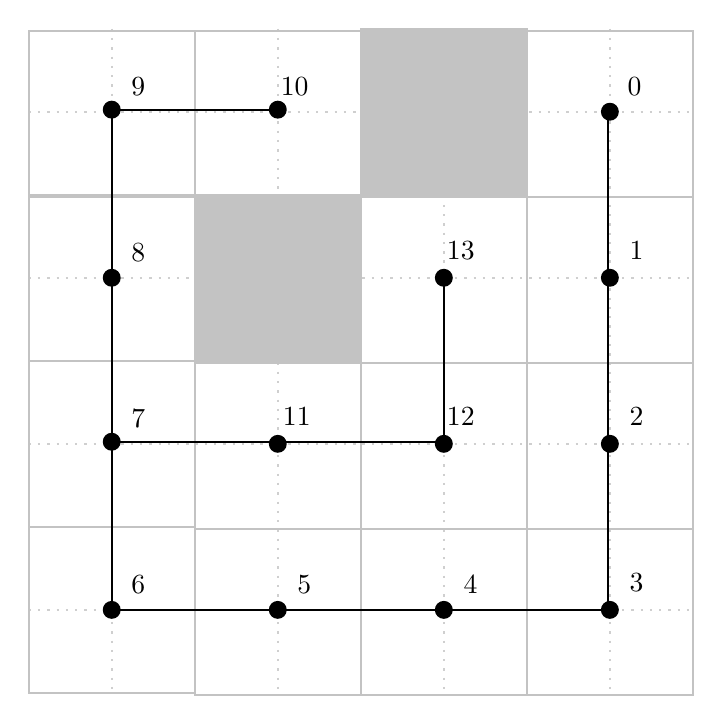
\begin{tikzpicture}[x=0.75pt,y=0.75pt,yscale=-1,xscale=1]
		%uncomment if require: \path (0,487); %set diagram left start at 0, and has height of 487
		
		%Straight Lines [id:da07078059737294629] 
		\draw [color={rgb, 255:red, 195; green, 195; blue, 195 }  ,draw opacity=0.8 ] [dash pattern={on 0.84pt off 2.51pt}]  (160,20) -- (160,340) ;
		%Straight Lines [id:da917458971819372] 
		\draw [color={rgb, 255:red, 195; green, 195; blue, 195 }  ,draw opacity=0.8 ] [dash pattern={on 0.84pt off 2.51pt}]  (240,20) -- (240,340) ;
		%Straight Lines [id:da8412450773677167] 
		\draw [color={rgb, 255:red, 195; green, 195; blue, 195 }  ,draw opacity=0.8 ] [dash pattern={on 0.84pt off 2.51pt}]  (320,20) -- (320,340) ;
		%Straight Lines [id:da3101903735332392] 
		\draw [color={rgb, 255:red, 195; green, 195; blue, 195 }  ,draw opacity=0.8 ] [dash pattern={on 0.84pt off 2.51pt}]  (400,20) -- (400,340) ;
		%Straight Lines [id:da43752561891339337] 
		\draw [color={rgb, 255:red, 195; green, 195; blue, 195 }  ,draw opacity=0.8 ] [dash pattern={on 0.84pt off 2.51pt}]  (120,60) -- (440,60) ;
		%Straight Lines [id:da21568167599612686] 
		\draw [color={rgb, 255:red, 195; green, 195; blue, 195 }  ,draw opacity=0.8 ] [dash pattern={on 0.84pt off 2.51pt}]  (120,140) -- (440,140) ;
		%Straight Lines [id:da9351274558937845] 
		\draw [color={rgb, 255:red, 195; green, 195; blue, 195 }  ,draw opacity=0.8 ] [dash pattern={on 0.84pt off 2.51pt}]  (120,220) -- (440,220) ;
		%Straight Lines [id:da8497636326794216] 
		\draw [color={rgb, 255:red, 195; green, 195; blue, 195 }  ,draw opacity=0.8 ] [dash pattern={on 0.84pt off 2.51pt}]  (120,300) -- (440,300) ;
		
		%Shape: Rectangle [id:dp7512840321055914] 
		\draw  [color={rgb, 255:red, 195; green, 195; blue, 195 }  ,draw opacity=1 ][line width=0.75]  (360,21) -- (440,21) -- (440,101) -- (360,101) -- cycle ;
		%Shape: Rectangle [id:dp08998875837998588] 
		\draw  [color={rgb, 255:red, 195; green, 195; blue, 195 }  ,draw opacity=1 ][line width=0.75]  (360,101) -- (440,101) -- (440,181) -- (360,181) -- cycle ;
		%Shape: Rectangle [id:dp0951355467677828] 
		\draw  [color={rgb, 255:red, 195; green, 195; blue, 195 }  ,draw opacity=1 ][line width=0.75]  (360,181) -- (440,181) -- (440,261) -- (360,261) -- cycle ;
		%Shape: Rectangle [id:dp7521114125139936] 
		\draw  [color={rgb, 255:red, 195; green, 195; blue, 195 }  ,draw opacity=1 ][line width=0.75]  (360,261) -- (440,261) -- (440,341) -- (360,341) -- cycle ;
		%Shape: Rectangle [id:dp7559961198567777] 
		\draw  [color={rgb, 255:red, 195; green, 195; blue, 195 }  ,draw opacity=1 ][line width=0.75]  (280,101) -- (360,101) -- (360,181) -- (280,181) -- cycle ;
		%Shape: Rectangle [id:dp8869961360769938] 
		\draw  [color={rgb, 255:red, 195; green, 195; blue, 195 }  ,draw opacity=1 ][line width=0.75]  (280,181) -- (360,181) -- (360,261) -- (280,261) -- cycle ;
		%Shape: Rectangle [id:dp5037977259529054] 
		\draw  [color={rgb, 255:red, 195; green, 195; blue, 195 }  ,draw opacity=1 ][line width=0.75]  (280,261) -- (360,261) -- (360,341) -- (280,341) -- cycle ;
		%Shape: Rectangle [id:dp773885446585411] 
		\draw  [color={rgb, 255:red, 195; green, 195; blue, 195 }  ,draw opacity=1 ][line width=0.75]  (200,21) -- (280,21) -- (280,101) -- (200,101) -- cycle ;
		%Shape: Rectangle [id:dp2052220638960709] 
		\draw  [color={rgb, 255:red, 195; green, 195; blue, 195 }  ,draw opacity=1 ][line width=0.75]  (120,21) -- (200,21) -- (200,101) -- (120,101) -- cycle ;
		%Shape: Rectangle [id:dp7105833624892055] 
		\draw  [color={rgb, 255:red, 195; green, 195; blue, 195 }  ,draw opacity=1 ][line width=0.75]  (120,100) -- (200,100) -- (200,180) -- (120,180) -- cycle ;
		%Shape: Rectangle [id:dp25180360725760975] 
		\draw  [color={rgb, 255:red, 195; green, 195; blue, 195 }  ,draw opacity=1 ][line width=0.75]  (120,180) -- (200,180) -- (200,260) -- (120,260) -- cycle ;
		%Shape: Rectangle [id:dp8614444924044413] 
		\draw  [color={rgb, 255:red, 195; green, 195; blue, 195 }  ,draw opacity=1 ][line width=0.75]  (120,260) -- (200,260) -- (200,340) -- (120,340) -- cycle ;
		%Shape: Rectangle [id:dp8378559698110666] 
		\draw  [color={rgb, 255:red, 195; green, 195; blue, 195 }  ,draw opacity=1 ][line width=0.75]  (200,181) -- (280,181) -- (280,261) -- (200,261) -- cycle ;
		%Shape: Rectangle [id:dp8380708528890195] 
		\draw  [color={rgb, 255:red, 195; green, 195; blue, 195 }  ,draw opacity=1 ][line width=0.75]  (200,261) -- (280,261) -- (280,341) -- (200,341) -- cycle ;
		
		%Straight Lines [id:da1979706309085778] 
		\draw [color={rgb, 255:red, 0; green, 0; blue, 0 }  ,draw opacity=1 ][line width=0.75]    (160,299) -- (160,59) ;
		%Shape: Rectangle [id:dp7251933800186736] 
		\draw  [color={rgb, 255:red, 195; green, 195; blue, 195 }  ,draw opacity=1 ][fill={rgb, 255:red, 195; green, 195; blue, 195 }  ,fill opacity=1 ][line width=0.75]  (280,20) -- (360,20) -- (360,100) -- (280,100) -- cycle ;
		%Shape: Rectangle [id:dp1925911620328833] 
		\draw  [color={rgb, 255:red, 195; green, 195; blue, 195 }  ,draw opacity=1 ][fill={rgb, 255:red, 195; green, 195; blue, 195 }  ,fill opacity=1 ][line width=0.75]  (200,100) -- (280,100) -- (280,180) -- (200,180) -- cycle ;
		%Straight Lines [id:da0581482096059478] 
		\draw [color={rgb, 255:red, 0; green, 0; blue, 0 }  ,draw opacity=1 ][line width=0.75]    (160,300) -- (400,300) ;
		%Straight Lines [id:da8084405416238001] 
		\draw [color={rgb, 255:red, 0; green, 0; blue, 0 }  ,draw opacity=1 ][line width=0.75]    (160,59) -- (240,59) ;
		%Straight Lines [id:da41325892147339616] 
		\draw [color={rgb, 255:red, 0; green, 0; blue, 0 }  ,draw opacity=1 ][fill={rgb, 255:red, 155; green, 155; blue, 155 }  ,fill opacity=1 ][line width=0.75]    (160,219) -- (320,219) ;
		%Straight Lines [id:da0985686119799063] 
		\draw [color={rgb, 255:red, 0; green, 0; blue, 0 }  ,draw opacity=1 ][line width=0.75]    (320,220) -- (320,140) ;
		%Straight Lines [id:da3298203658421879] 
		\draw [color={rgb, 255:red, 0; green, 0; blue, 0 }  ,draw opacity=1 ][line width=0.75]    (399,300) -- (399,60) ;
		%Shape: Circle [id:dp41582492626714096] 
		\draw  [color={rgb, 255:red, 0; green, 0; blue, 0 }  ,draw opacity=1 ][fill={rgb, 255:red, 0; green, 0; blue, 0 }  ,fill opacity=1 ] (236.19,59) .. controls (236.19,56.89) and (237.89,55.19) .. (240,55.19) .. controls (242.11,55.19) and (243.81,56.89) .. (243.81,59) .. controls (243.81,61.11) and (242.11,62.81) .. (240,62.81) .. controls (237.89,62.81) and (236.19,61.11) .. (236.19,59) -- cycle ;
		%Shape: Circle [id:dp5558894380647834] 
		\draw  [color={rgb, 255:red, 0; green, 0; blue, 0 }  ,draw opacity=1 ][fill={rgb, 255:red, 0; green, 0; blue, 0 }  ,fill opacity=1 ] (156.19,59) .. controls (156.19,56.89) and (157.89,55.19) .. (160,55.19) .. controls (162.11,55.19) and (163.81,56.89) .. (163.81,59) .. controls (163.81,61.11) and (162.11,62.81) .. (160,62.81) .. controls (157.89,62.81) and (156.19,61.11) .. (156.19,59) -- cycle ;
		%Shape: Circle [id:dp8351577385814617] 
		\draw  [color={rgb, 255:red, 0; green, 0; blue, 0 }  ,draw opacity=1 ][fill={rgb, 255:red, 0; green, 0; blue, 0 }  ,fill opacity=1 ] (396.19,60) .. controls (396.19,57.89) and (397.89,56.19) .. (400,56.19) .. controls (402.11,56.19) and (403.81,57.89) .. (403.81,60) .. controls (403.81,62.11) and (402.11,63.81) .. (400,63.81) .. controls (397.89,63.81) and (396.19,62.11) .. (396.19,60) -- cycle ;
		%Shape: Circle [id:dp7940426606232267] 
		\draw  [color={rgb, 255:red, 0; green, 0; blue, 0 }  ,draw opacity=1 ][fill={rgb, 255:red, 0; green, 0; blue, 0 }  ,fill opacity=1 ] (316.19,140) .. controls (316.19,137.89) and (317.89,136.19) .. (320,136.19) .. controls (322.11,136.19) and (323.81,137.89) .. (323.81,140) .. controls (323.81,142.11) and (322.11,143.81) .. (320,143.81) .. controls (317.89,143.81) and (316.19,142.11) .. (316.19,140) -- cycle ;
		%Shape: Circle [id:dp04520481160188616] 
		\draw  [color={rgb, 255:red, 0; green, 0; blue, 0 }  ,draw opacity=1 ][fill={rgb, 255:red, 0; green, 0; blue, 0 }  ,fill opacity=1 ] (316.19,220) .. controls (316.19,217.89) and (317.89,216.19) .. (320,216.19) .. controls (322.11,216.19) and (323.81,217.89) .. (323.81,220) .. controls (323.81,222.11) and (322.11,223.81) .. (320,223.81) .. controls (317.89,223.81) and (316.19,222.11) .. (316.19,220) -- cycle ;
		%Shape: Circle [id:dp5073699623939971] 
		\draw  [color={rgb, 255:red, 0; green, 0; blue, 0 }  ,draw opacity=1 ][fill={rgb, 255:red, 0; green, 0; blue, 0 }  ,fill opacity=1 ] (236.19,220) .. controls (236.19,217.89) and (237.89,216.19) .. (240,216.19) .. controls (242.11,216.19) and (243.81,217.89) .. (243.81,220) .. controls (243.81,222.11) and (242.11,223.81) .. (240,223.81) .. controls (237.89,223.81) and (236.19,222.11) .. (236.19,220) -- cycle ;
		%Shape: Circle [id:dp2213240590117067] 
		\draw  [color={rgb, 255:red, 0; green, 0; blue, 0 }  ,draw opacity=1 ][fill={rgb, 255:red, 0; green, 0; blue, 0 }  ,fill opacity=1 ] (156.19,219) .. controls (156.19,216.89) and (157.89,215.19) .. (160,215.19) .. controls (162.11,215.19) and (163.81,216.89) .. (163.81,219) .. controls (163.81,221.11) and (162.11,222.81) .. (160,222.81) .. controls (157.89,222.81) and (156.19,221.11) .. (156.19,219) -- cycle ;
		%Shape: Circle [id:dp979294341687238] 
		\draw  [color={rgb, 255:red, 0; green, 0; blue, 0 }  ,draw opacity=1 ][fill={rgb, 255:red, 0; green, 0; blue, 0 }  ,fill opacity=1 ] (156.19,140) .. controls (156.19,137.89) and (157.89,136.19) .. (160,136.19) .. controls (162.11,136.19) and (163.81,137.89) .. (163.81,140) .. controls (163.81,142.11) and (162.11,143.81) .. (160,143.81) .. controls (157.89,143.81) and (156.19,142.11) .. (156.19,140) -- cycle ;
		%Shape: Circle [id:dp14676659616041077] 
		\draw  [color={rgb, 255:red, 0; green, 0; blue, 0 }  ,draw opacity=1 ][fill={rgb, 255:red, 0; green, 0; blue, 0 }  ,fill opacity=1 ] (396.19,140) .. controls (396.19,137.89) and (397.89,136.19) .. (400,136.19) .. controls (402.11,136.19) and (403.81,137.89) .. (403.81,140) .. controls (403.81,142.11) and (402.11,143.81) .. (400,143.81) .. controls (397.89,143.81) and (396.19,142.11) .. (396.19,140) -- cycle ;
		%Shape: Circle [id:dp19334338983125243] 
		\draw  [color={rgb, 255:red, 0; green, 0; blue, 0 }  ,draw opacity=1 ][fill={rgb, 255:red, 0; green, 0; blue, 0 }  ,fill opacity=1 ] (396.19,220) .. controls (396.19,217.89) and (397.89,216.19) .. (400,216.19) .. controls (402.11,216.19) and (403.81,217.89) .. (403.81,220) .. controls (403.81,222.11) and (402.11,223.81) .. (400,223.81) .. controls (397.89,223.81) and (396.19,222.11) .. (396.19,220) -- cycle ;
		%Shape: Circle [id:dp5263269612866854] 
		\draw  [color={rgb, 255:red, 0; green, 0; blue, 0 }  ,draw opacity=1 ][fill={rgb, 255:red, 0; green, 0; blue, 0 }  ,fill opacity=1 ] (396.19,300) .. controls (396.19,297.89) and (397.89,296.19) .. (400,296.19) .. controls (402.11,296.19) and (403.81,297.89) .. (403.81,300) .. controls (403.81,302.11) and (402.11,303.81) .. (400,303.81) .. controls (397.89,303.81) and (396.19,302.11) .. (396.19,300) -- cycle ;
		%Shape: Circle [id:dp41455563786620653] 
		\draw  [color={rgb, 255:red, 0; green, 0; blue, 0 }  ,draw opacity=1 ][fill={rgb, 255:red, 0; green, 0; blue, 0 }  ,fill opacity=1 ] (316.19,300) .. controls (316.19,297.89) and (317.89,296.19) .. (320,296.19) .. controls (322.11,296.19) and (323.81,297.89) .. (323.81,300) .. controls (323.81,302.11) and (322.11,303.81) .. (320,303.81) .. controls (317.89,303.81) and (316.19,302.11) .. (316.19,300) -- cycle ;
		%Shape: Circle [id:dp9746259257783465] 
		\draw  [color={rgb, 255:red, 0; green, 0; blue, 0 }  ,draw opacity=1 ][fill={rgb, 255:red, 0; green, 0; blue, 0 }  ,fill opacity=1 ] (236.19,300) .. controls (236.19,297.89) and (237.89,296.19) .. (240,296.19) .. controls (242.11,296.19) and (243.81,297.89) .. (243.81,300) .. controls (243.81,302.11) and (242.11,303.81) .. (240,303.81) .. controls (237.89,303.81) and (236.19,302.11) .. (236.19,300) -- cycle ;
		%Shape: Circle [id:dp5753636930291428] 
		\draw  [color={rgb, 255:red, 0; green, 0; blue, 0 }  ,draw opacity=1 ][fill={rgb, 255:red, 0; green, 0; blue, 0 }  ,fill opacity=1 ] (156.19,300) .. controls (156.19,297.89) and (157.89,296.19) .. (160,296.19) .. controls (162.11,296.19) and (163.81,297.89) .. (163.81,300) .. controls (163.81,302.11) and (162.11,303.81) .. (160,303.81) .. controls (157.89,303.81) and (156.19,302.11) .. (156.19,300) -- cycle ;
		
		% Text Node
		\draw (407,42) node [anchor=north west][inner sep=0.75pt]   [align=left] {0};
		% Text Node
		\draw (408,121) node [anchor=north west][inner sep=0.75pt]   [align=left] {1};
		% Text Node
		\draw (408,201) node [anchor=north west][inner sep=0.75pt]   [align=left] {2};
		% Text Node
		\draw (408,281) node [anchor=north west][inner sep=0.75pt]   [align=left] {3};
		% Text Node
		\draw (328,282) node [anchor=north west][inner sep=0.75pt]   [align=left] {4};
		% Text Node
		\draw (248,282) node [anchor=north west][inner sep=0.75pt]   [align=left] {5};
		% Text Node
		\draw (168,282) node [anchor=north west][inner sep=0.75pt]   [align=left] {6};
		% Text Node
		\draw (168,202) node [anchor=north west][inner sep=0.75pt]   [align=left] {7};
		% Text Node
		\draw (168,122) node [anchor=north west][inner sep=0.75pt]   [align=left] {8};
		% Text Node
		\draw (168,42) node [anchor=north west][inner sep=0.75pt]   [align=left] {9};
		% Text Node
		\draw (240,42) node [anchor=north west][inner sep=0.75pt]   [align=left] {10};
		% Text Node
		\draw (241,201) node [anchor=north west][inner sep=0.75pt]   [align=left] {11};
		% Text Node
		\draw (320,201) node [anchor=north west][inner sep=0.75pt]   [align=left] {12};
		% Text Node
		\draw (320,121) node [anchor=north west][inner sep=0.75pt]   [align=left] {13};
		
		
	\end{tikzpicture}
	\caption{Figure showing a spanning tree generated for a four-by-four environment grid}
	\label{fig:grid-st}
\end{figure}

\begin{figure}[h!]
	\centering
	\tikzset{every picture/.style={line width=0.75pt}} %set default line width to 0.75pt        
	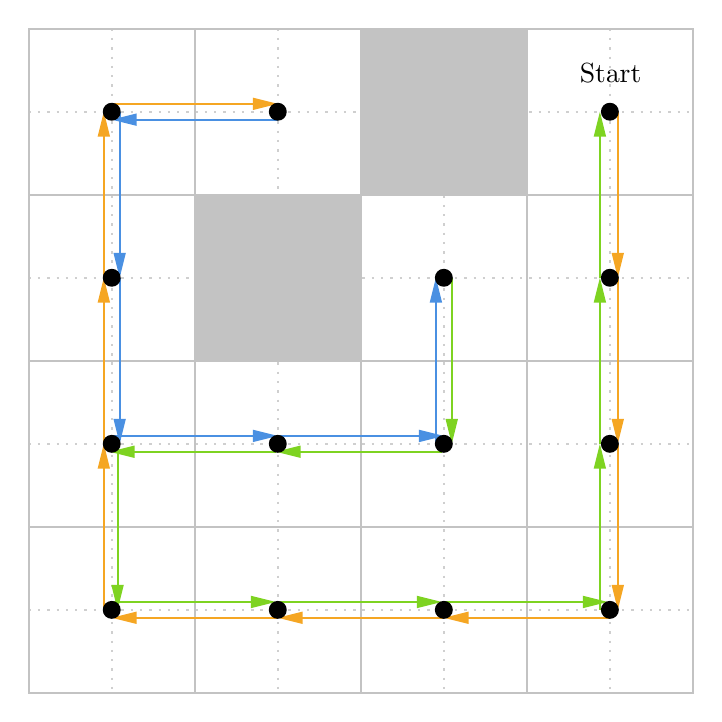
\begin{tikzpicture}[x=0.75pt,y=0.75pt,yscale=-1,xscale=1]
		%uncomment if require: \path (0,487); %set diagram left start at 0, and has height of 487
		
		%Straight Lines [id:da3977750045093258] 
		\draw [color={rgb, 255:red, 195; green, 195; blue, 195 }  ,draw opacity=0.8 ] [dash pattern={on 0.84pt off 2.51pt}]  (160,20) -- (160,340) ;
		%Straight Lines [id:da07618883915401731] 
		\draw [color={rgb, 255:red, 195; green, 195; blue, 195 }  ,draw opacity=0.8 ] [dash pattern={on 0.84pt off 2.51pt}]  (240,20) -- (240,340) ;
		%Straight Lines [id:da06600432409341517] 
		\draw [color={rgb, 255:red, 195; green, 195; blue, 195 }  ,draw opacity=0.8 ] [dash pattern={on 0.84pt off 2.51pt}]  (320,20) -- (320,340) ;
		%Straight Lines [id:da5290784258779333] 
		\draw [color={rgb, 255:red, 195; green, 195; blue, 195 }  ,draw opacity=0.8 ] [dash pattern={on 0.84pt off 2.51pt}]  (400,20) -- (400,340) ;
		%Straight Lines [id:da9833595064287617] 
		\draw [color={rgb, 255:red, 195; green, 195; blue, 195 }  ,draw opacity=0.8 ] [dash pattern={on 0.84pt off 2.51pt}]  (120,60) -- (440,60) ;
		%Straight Lines [id:da520432231001738] 
		\draw [color={rgb, 255:red, 195; green, 195; blue, 195 }  ,draw opacity=0.8 ] [dash pattern={on 0.84pt off 2.51pt}]  (120,140) -- (440,140) ;
		%Straight Lines [id:da6002867106183594] 
		\draw [color={rgb, 255:red, 195; green, 195; blue, 195 }  ,draw opacity=0.8 ] [dash pattern={on 0.84pt off 2.51pt}]  (120,220) -- (440,220) ;
		%Straight Lines [id:da9782745721301296] 
		\draw [color={rgb, 255:red, 195; green, 195; blue, 195 }  ,draw opacity=0.8 ] [dash pattern={on 0.84pt off 2.51pt}]  (120,300) -- (440,300) ;
		
		%Shape: Rectangle [id:dp5898184612923194] 
		\draw  [color={rgb, 255:red, 195; green, 195; blue, 195 }  ,draw opacity=1 ][line width=0.75]  (360,20) -- (440,20) -- (440,100) -- (360,100) -- cycle ;
		%Shape: Rectangle [id:dp48862096625716034] 
		\draw  [color={rgb, 255:red, 195; green, 195; blue, 195 }  ,draw opacity=1 ][line width=0.75]  (360,100) -- (440,100) -- (440,180) -- (360,180) -- cycle ;
		%Shape: Rectangle [id:dp3755148108063808] 
		\draw  [color={rgb, 255:red, 195; green, 195; blue, 195 }  ,draw opacity=1 ][line width=0.75]  (360,180) -- (440,180) -- (440,260) -- (360,260) -- cycle ;
		%Shape: Rectangle [id:dp9473736210218475] 
		\draw  [color={rgb, 255:red, 195; green, 195; blue, 195 }  ,draw opacity=1 ][line width=0.75]  (360,260) -- (440,260) -- (440,340) -- (360,340) -- cycle ;
		%Shape: Rectangle [id:dp12436408430349899] 
		\draw  [color={rgb, 255:red, 195; green, 195; blue, 195 }  ,draw opacity=1 ][line width=0.75]  (280,100) -- (360,100) -- (360,180) -- (280,180) -- cycle ;
		%Shape: Rectangle [id:dp43828113255227175] 
		\draw  [color={rgb, 255:red, 195; green, 195; blue, 195 }  ,draw opacity=1 ][line width=0.75]  (280,180) -- (360,180) -- (360,260) -- (280,260) -- cycle ;
		%Shape: Rectangle [id:dp7405502584040733] 
		\draw  [color={rgb, 255:red, 195; green, 195; blue, 195 }  ,draw opacity=1 ][line width=0.75]  (280,260) -- (360,260) -- (360,340) -- (280,340) -- cycle ;
		%Shape: Rectangle [id:dp05296394236381641] 
		\draw  [color={rgb, 255:red, 195; green, 195; blue, 195 }  ,draw opacity=1 ][line width=0.75]  (120,20) -- (200,20) -- (200,100) -- (120,100) -- cycle ;
		%Shape: Rectangle [id:dp6150857421701121] 
		\draw  [color={rgb, 255:red, 195; green, 195; blue, 195 }  ,draw opacity=1 ][line width=0.75]  (120,100) -- (200,100) -- (200,180) -- (120,180) -- cycle ;
		%Shape: Rectangle [id:dp5861189397744904] 
		\draw  [color={rgb, 255:red, 195; green, 195; blue, 195 }  ,draw opacity=1 ][line width=0.75]  (120,180) -- (200,180) -- (200,260) -- (120,260) -- cycle ;
		%Shape: Rectangle [id:dp8672396938760043] 
		\draw  [color={rgb, 255:red, 195; green, 195; blue, 195 }  ,draw opacity=1 ][line width=0.75]  (120,260) -- (200,260) -- (200,340) -- (120,340) -- cycle ;
		%Shape: Rectangle [id:dp32997979058045] 
		\draw  [color={rgb, 255:red, 195; green, 195; blue, 195 }  ,draw opacity=1 ][line width=0.75]  (200,180) -- (280,180) -- (280,260) -- (200,260) -- cycle ;
		%Shape: Rectangle [id:dp6083880745681156] 
		\draw  [color={rgb, 255:red, 195; green, 195; blue, 195 }  ,draw opacity=1 ][line width=0.75]  (200,260) -- (280,260) -- (280,340) -- (200,340) -- cycle ;
		
		%Shape: Rectangle [id:dp6989257767580808] 
		\draw  [color={rgb, 255:red, 195; green, 195; blue, 195 }  ,draw opacity=1 ][line width=0.75]  (200,20) -- (280,20) -- (280,100) -- (200,100) -- cycle ;
		
		%Shape: Rectangle [id:dp3496282639540844] 
		\draw  [color={rgb, 255:red, 195; green, 195; blue, 195 }  ,draw opacity=1 ][fill={rgb, 255:red, 195; green, 195; blue, 195 }  ,fill opacity=1 ][line width=0.75]  (280,20) -- (360,20) -- (360,100) -- (280,100) -- cycle ;
		%Shape: Rectangle [id:dp1101274608527989] 
		\draw  [color={rgb, 255:red, 195; green, 195; blue, 195 }  ,draw opacity=1 ][fill={rgb, 255:red, 195; green, 195; blue, 195 }  ,fill opacity=1 ][line width=0.75]  (200,100) -- (280,100) -- (280,180) -- (200,180) -- cycle ;
		%Straight Lines [id:da7109877053031188] 
		\draw [color={rgb, 255:red, 245; green, 166; blue, 35 }  ,draw opacity=1 ]   (403.81,60) -- (403.81,138) ;
		\draw [shift={(403.81,140)}, rotate = 270] [fill={rgb, 255:red, 245; green, 166; blue, 35 }  ,fill opacity=1 ][line width=0.08]  [draw opacity=0] (12,-3) -- (0,0) -- (12,3) -- cycle    ;
		%Straight Lines [id:da26602598944672584] 
		\draw [color={rgb, 255:red, 126; green, 211; blue, 33 }  ,draw opacity=1 ]   (395.19,140) -- (395.19,62) ;
		\draw [shift={(395.19,60)}, rotate = 450] [fill={rgb, 255:red, 126; green, 211; blue, 33 }  ,fill opacity=1 ][line width=0.08]  [draw opacity=0] (12,-3) -- (0,0) -- (12,3) -- cycle    ;
		%Straight Lines [id:da02914591351940765] 
		\draw [color={rgb, 255:red, 126; green, 211; blue, 33 }  ,draw opacity=1 ]   (395.19,220) -- (395.19,142) ;
		\draw [shift={(395.19,140)}, rotate = 450] [fill={rgb, 255:red, 126; green, 211; blue, 33 }  ,fill opacity=1 ][line width=0.08]  [draw opacity=0] (12,-3) -- (0,0) -- (12,3) -- cycle    ;
		%Straight Lines [id:da39308513285178037] 
		\draw [color={rgb, 255:red, 245; green, 166; blue, 35 }  ,draw opacity=1 ]   (403.81,140) -- (403.81,218) ;
		\draw [shift={(403.81,220)}, rotate = 270] [fill={rgb, 255:red, 245; green, 166; blue, 35 }  ,fill opacity=1 ][line width=0.08]  [draw opacity=0] (12,-3) -- (0,0) -- (12,3) -- cycle    ;
		%Straight Lines [id:da5373248798431745] 
		\draw [color={rgb, 255:red, 245; green, 166; blue, 35 }  ,draw opacity=1 ]   (403.81,220) -- (403.81,298) ;
		\draw [shift={(403.81,300)}, rotate = 270] [fill={rgb, 255:red, 245; green, 166; blue, 35 }  ,fill opacity=1 ][line width=0.08]  [draw opacity=0] (12,-3) -- (0,0) -- (12,3) -- cycle    ;
		%Straight Lines [id:da6507397451478356] 
		\draw [color={rgb, 255:red, 126; green, 211; blue, 33 }  ,draw opacity=1 ]   (395.19,300) -- (395.19,222) ;
		\draw [shift={(395.19,220)}, rotate = 450] [fill={rgb, 255:red, 126; green, 211; blue, 33 }  ,fill opacity=1 ][line width=0.08]  [draw opacity=0] (12,-3) -- (0,0) -- (12,3) -- cycle    ;
		%Straight Lines [id:da4490944583331955] 
		\draw [color={rgb, 255:red, 245; green, 166; blue, 35 }  ,draw opacity=1 ]   (400,303.81) -- (322,303.81) ;
		\draw [shift={(320,303.81)}, rotate = 360] [fill={rgb, 255:red, 245; green, 166; blue, 35 }  ,fill opacity=1 ][line width=0.08]  [draw opacity=0] (12,-3) -- (0,0) -- (12,3) -- cycle    ;
		%Straight Lines [id:da771333880279802] 
		\draw [color={rgb, 255:red, 245; green, 166; blue, 35 }  ,draw opacity=1 ]   (320,303.81) -- (242,303.81) ;
		\draw [shift={(240,303.81)}, rotate = 360] [fill={rgb, 255:red, 245; green, 166; blue, 35 }  ,fill opacity=1 ][line width=0.08]  [draw opacity=0] (12,-3) -- (0,0) -- (12,3) -- cycle    ;
		%Straight Lines [id:da0915527602751669] 
		\draw [color={rgb, 255:red, 245; green, 166; blue, 35 }  ,draw opacity=1 ]   (240,303.81) -- (162,303.81) ;
		\draw [shift={(160,303.81)}, rotate = 360] [fill={rgb, 255:red, 245; green, 166; blue, 35 }  ,fill opacity=1 ][line width=0.08]  [draw opacity=0] (12,-3) -- (0,0) -- (12,3) -- cycle    ;
		%Straight Lines [id:da8183550519262464] 
		\draw [color={rgb, 255:red, 126; green, 211; blue, 33 }  ,draw opacity=1 ]   (319,296.19) -- (397,296.19) ;
		\draw [shift={(399,296.19)}, rotate = 180] [fill={rgb, 255:red, 126; green, 211; blue, 33 }  ,fill opacity=1 ][line width=0.08]  [draw opacity=0] (12,-3) -- (0,0) -- (12,3) -- cycle    ;
		%Straight Lines [id:da270699769832347] 
		\draw [color={rgb, 255:red, 126; green, 211; blue, 33 }  ,draw opacity=1 ]   (239,296.19) -- (317,296.19) ;
		\draw [shift={(319,296.19)}, rotate = 180] [fill={rgb, 255:red, 126; green, 211; blue, 33 }  ,fill opacity=1 ][line width=0.08]  [draw opacity=0] (12,-3) -- (0,0) -- (12,3) -- cycle    ;
		%Straight Lines [id:da5296508036432168] 
		\draw [color={rgb, 255:red, 126; green, 211; blue, 33 }  ,draw opacity=1 ]   (159,296.19) -- (237,296.19) ;
		\draw [shift={(239,296.19)}, rotate = 180] [fill={rgb, 255:red, 126; green, 211; blue, 33 }  ,fill opacity=1 ][line width=0.08]  [draw opacity=0] (12,-3) -- (0,0) -- (12,3) -- cycle    ;
		%Straight Lines [id:da6152908850819139] 
		\draw [color={rgb, 255:red, 245; green, 166; blue, 35 }  ,draw opacity=1 ]   (156.19,300) -- (156.19,222) ;
		\draw [shift={(156.19,220)}, rotate = 450] [fill={rgb, 255:red, 245; green, 166; blue, 35 }  ,fill opacity=1 ][line width=0.08]  [draw opacity=0] (12,-3) -- (0,0) -- (12,3) -- cycle    ;
		%Straight Lines [id:da4869759720464193] 
		\draw [color={rgb, 255:red, 245; green, 166; blue, 35 }  ,draw opacity=1 ]   (160,56.19) -- (238,56.19) ;
		\draw [shift={(240,56.19)}, rotate = 180] [fill={rgb, 255:red, 245; green, 166; blue, 35 }  ,fill opacity=1 ][line width=0.08]  [draw opacity=0] (12,-3) -- (0,0) -- (12,3) -- cycle    ;
		%Straight Lines [id:da41392688240238984] 
		\draw [color={rgb, 255:red, 74; green, 144; blue, 226 }  ,draw opacity=1 ]   (240,63.81) -- (162,63.81) ;
		\draw [shift={(160,63.81)}, rotate = 360] [fill={rgb, 255:red, 74; green, 144; blue, 226 }  ,fill opacity=1 ][line width=0.08]  [draw opacity=0] (12,-3) -- (0,0) -- (12,3) -- cycle    ;
		%Straight Lines [id:da1371170506661339] 
		\draw [color={rgb, 255:red, 126; green, 211; blue, 33 }  ,draw opacity=1 ]   (162.81,220) -- (162.81,298) ;
		\draw [shift={(162.81,300)}, rotate = 270] [fill={rgb, 255:red, 126; green, 211; blue, 33 }  ,fill opacity=1 ][line width=0.08]  [draw opacity=0] (12,-3) -- (0,0) -- (12,3) -- cycle    ;
		%Straight Lines [id:da06913212613382202] 
		\draw [color={rgb, 255:red, 74; green, 144; blue, 226 }  ,draw opacity=1 ]   (160,216.19) -- (238,216.19) ;
		\draw [shift={(240,216.19)}, rotate = 180] [fill={rgb, 255:red, 74; green, 144; blue, 226 }  ,fill opacity=1 ][line width=0.08]  [draw opacity=0] (12,-3) -- (0,0) -- (12,3) -- cycle    ;
		%Straight Lines [id:da37746092338955006] 
		\draw [color={rgb, 255:red, 126; green, 211; blue, 33 }  ,draw opacity=1 ]   (239,223.81) -- (161,223.81) ;
		\draw [shift={(159,223.81)}, rotate = 360] [fill={rgb, 255:red, 126; green, 211; blue, 33 }  ,fill opacity=1 ][line width=0.08]  [draw opacity=0] (12,-3) -- (0,0) -- (12,3) -- cycle    ;
		%Straight Lines [id:da5502420093118436] 
		\draw [color={rgb, 255:red, 126; green, 211; blue, 33 }  ,draw opacity=1 ]   (319,223.81) -- (241,223.81) ;
		\draw [shift={(239,223.81)}, rotate = 360] [fill={rgb, 255:red, 126; green, 211; blue, 33 }  ,fill opacity=1 ][line width=0.08]  [draw opacity=0] (12,-3) -- (0,0) -- (12,3) -- cycle    ;
		%Straight Lines [id:da25223475086499536] 
		\draw [color={rgb, 255:red, 74; green, 144; blue, 226 }  ,draw opacity=1 ]   (240,216.19) -- (318,216.19) ;
		\draw [shift={(320,216.19)}, rotate = 180] [fill={rgb, 255:red, 74; green, 144; blue, 226 }  ,fill opacity=1 ][line width=0.08]  [draw opacity=0] (12,-3) -- (0,0) -- (12,3) -- cycle    ;
		%Straight Lines [id:da8200476146784395] 
		\draw [color={rgb, 255:red, 74; green, 144; blue, 226 }  ,draw opacity=1 ]   (316.19,220) -- (316.19,142) ;
		\draw [shift={(316.19,140)}, rotate = 450] [fill={rgb, 255:red, 74; green, 144; blue, 226 }  ,fill opacity=1 ][line width=0.08]  [draw opacity=0] (12,-3) -- (0,0) -- (12,3) -- cycle    ;
		%Straight Lines [id:da5178980162476476] 
		\draw [color={rgb, 255:red, 126; green, 211; blue, 33 }  ,draw opacity=1 ]   (323.81,140) -- (323.81,218) ;
		\draw [shift={(323.81,220)}, rotate = 270] [fill={rgb, 255:red, 126; green, 211; blue, 33 }  ,fill opacity=1 ][line width=0.08]  [draw opacity=0] (12,-3) -- (0,0) -- (12,3) -- cycle    ;
		%Straight Lines [id:da5994423368626156] 
		\draw [color={rgb, 255:red, 245; green, 166; blue, 35 }  ,draw opacity=1 ]   (156.19,220) -- (156.19,142) ;
		\draw [shift={(156.19,140)}, rotate = 450] [fill={rgb, 255:red, 245; green, 166; blue, 35 }  ,fill opacity=1 ][line width=0.08]  [draw opacity=0] (12,-3) -- (0,0) -- (12,3) -- cycle    ;
		%Straight Lines [id:da2748369034984963] 
		\draw [color={rgb, 255:red, 74; green, 144; blue, 226 }  ,draw opacity=1 ]   (163.81,140) -- (163.81,218) ;
		\draw [shift={(163.81,220)}, rotate = 270] [fill={rgb, 255:red, 74; green, 144; blue, 226 }  ,fill opacity=1 ][line width=0.08]  [draw opacity=0] (12,-3) -- (0,0) -- (12,3) -- cycle    ;
		%Straight Lines [id:da6753173854185068] 
		\draw [color={rgb, 255:red, 74; green, 144; blue, 226 }  ,draw opacity=1 ]   (163.81,60) -- (163.81,138) ;
		\draw [shift={(163.81,140)}, rotate = 270] [fill={rgb, 255:red, 74; green, 144; blue, 226 }  ,fill opacity=1 ][line width=0.08]  [draw opacity=0] (12,-3) -- (0,0) -- (12,3) -- cycle    ;
		%Straight Lines [id:da6119419475380783] 
		\draw [color={rgb, 255:red, 245; green, 166; blue, 35 }  ,draw opacity=1 ]   (156.19,140) -- (156.19,62) ;
		\draw [shift={(156.19,60)}, rotate = 450] [fill={rgb, 255:red, 245; green, 166; blue, 35 }  ,fill opacity=1 ][line width=0.08]  [draw opacity=0] (12,-3) -- (0,0) -- (12,3) -- cycle    ;
		%Shape: Circle [id:dp5879652604634542] 
		\draw  [color={rgb, 255:red, 0; green, 0; blue, 0 }  ,draw opacity=1 ][fill={rgb, 255:red, 0; green, 0; blue, 0 }  ,fill opacity=1 ] (236.19,60) .. controls (236.19,57.89) and (237.89,56.19) .. (240,56.19) .. controls (242.11,56.19) and (243.81,57.89) .. (243.81,60) .. controls (243.81,62.11) and (242.11,63.81) .. (240,63.81) .. controls (237.89,63.81) and (236.19,62.11) .. (236.19,60) -- cycle ;
		%Shape: Circle [id:dp818491645062577] 
		\draw  [color={rgb, 255:red, 0; green, 0; blue, 0 }  ,draw opacity=1 ][fill={rgb, 255:red, 0; green, 0; blue, 0 }  ,fill opacity=1 ] (156.19,60) .. controls (156.19,57.89) and (157.89,56.19) .. (160,56.19) .. controls (162.11,56.19) and (163.81,57.89) .. (163.81,60) .. controls (163.81,62.11) and (162.11,63.81) .. (160,63.81) .. controls (157.89,63.81) and (156.19,62.11) .. (156.19,60) -- cycle ;
		%Shape: Circle [id:dp16964786331372994] 
		\draw  [color={rgb, 255:red, 0; green, 0; blue, 0 }  ,draw opacity=1 ][fill={rgb, 255:red, 0; green, 0; blue, 0 }  ,fill opacity=1 ] (396.19,60) .. controls (396.19,57.89) and (397.89,56.19) .. (400,56.19) .. controls (402.11,56.19) and (403.81,57.89) .. (403.81,60) .. controls (403.81,62.11) and (402.11,63.81) .. (400,63.81) .. controls (397.89,63.81) and (396.19,62.11) .. (396.19,60) -- cycle ;
		%Shape: Circle [id:dp12685321021069051] 
		\draw  [color={rgb, 255:red, 0; green, 0; blue, 0 }  ,draw opacity=1 ][fill={rgb, 255:red, 0; green, 0; blue, 0 }  ,fill opacity=1 ] (316.19,140) .. controls (316.19,137.89) and (317.89,136.19) .. (320,136.19) .. controls (322.11,136.19) and (323.81,137.89) .. (323.81,140) .. controls (323.81,142.11) and (322.11,143.81) .. (320,143.81) .. controls (317.89,143.81) and (316.19,142.11) .. (316.19,140) -- cycle ;
		%Shape: Circle [id:dp14500238655020814] 
		\draw  [color={rgb, 255:red, 0; green, 0; blue, 0 }  ,draw opacity=1 ][fill={rgb, 255:red, 0; green, 0; blue, 0 }  ,fill opacity=1 ] (316.19,220) .. controls (316.19,217.89) and (317.89,216.19) .. (320,216.19) .. controls (322.11,216.19) and (323.81,217.89) .. (323.81,220) .. controls (323.81,222.11) and (322.11,223.81) .. (320,223.81) .. controls (317.89,223.81) and (316.19,222.11) .. (316.19,220) -- cycle ;
		%Shape: Circle [id:dp007101657201895817] 
		\draw  [color={rgb, 255:red, 0; green, 0; blue, 0 }  ,draw opacity=1 ][fill={rgb, 255:red, 0; green, 0; blue, 0 }  ,fill opacity=1 ] (236.19,220) .. controls (236.19,217.89) and (237.89,216.19) .. (240,216.19) .. controls (242.11,216.19) and (243.81,217.89) .. (243.81,220) .. controls (243.81,222.11) and (242.11,223.81) .. (240,223.81) .. controls (237.89,223.81) and (236.19,222.11) .. (236.19,220) -- cycle ;
		%Shape: Circle [id:dp19397915406266075] 
		\draw  [color={rgb, 255:red, 0; green, 0; blue, 0 }  ,draw opacity=1 ][fill={rgb, 255:red, 0; green, 0; blue, 0 }  ,fill opacity=1 ] (156.19,220) .. controls (156.19,217.89) and (157.89,216.19) .. (160,216.19) .. controls (162.11,216.19) and (163.81,217.89) .. (163.81,220) .. controls (163.81,222.11) and (162.11,223.81) .. (160,223.81) .. controls (157.89,223.81) and (156.19,222.11) .. (156.19,220) -- cycle ;
		%Shape: Circle [id:dp11650504808251783] 
		\draw  [color={rgb, 255:red, 0; green, 0; blue, 0 }  ,draw opacity=1 ][fill={rgb, 255:red, 0; green, 0; blue, 0 }  ,fill opacity=1 ] (156.19,140) .. controls (156.19,137.89) and (157.89,136.19) .. (160,136.19) .. controls (162.11,136.19) and (163.81,137.89) .. (163.81,140) .. controls (163.81,142.11) and (162.11,143.81) .. (160,143.81) .. controls (157.89,143.81) and (156.19,142.11) .. (156.19,140) -- cycle ;
		%Shape: Circle [id:dp14621496623583385] 
		\draw  [color={rgb, 255:red, 0; green, 0; blue, 0 }  ,draw opacity=1 ][fill={rgb, 255:red, 0; green, 0; blue, 0 }  ,fill opacity=1 ] (396.19,140) .. controls (396.19,137.89) and (397.89,136.19) .. (400,136.19) .. controls (402.11,136.19) and (403.81,137.89) .. (403.81,140) .. controls (403.81,142.11) and (402.11,143.81) .. (400,143.81) .. controls (397.89,143.81) and (396.19,142.11) .. (396.19,140) -- cycle ;
		%Shape: Circle [id:dp4178077365658106] 
		\draw  [color={rgb, 255:red, 0; green, 0; blue, 0 }  ,draw opacity=1 ][fill={rgb, 255:red, 0; green, 0; blue, 0 }  ,fill opacity=1 ] (396.19,220) .. controls (396.19,217.89) and (397.89,216.19) .. (400,216.19) .. controls (402.11,216.19) and (403.81,217.89) .. (403.81,220) .. controls (403.81,222.11) and (402.11,223.81) .. (400,223.81) .. controls (397.89,223.81) and (396.19,222.11) .. (396.19,220) -- cycle ;
		%Shape: Circle [id:dp5805338448968826] 
		\draw  [color={rgb, 255:red, 0; green, 0; blue, 0 }  ,draw opacity=1 ][fill={rgb, 255:red, 0; green, 0; blue, 0 }  ,fill opacity=1 ] (396.19,300) .. controls (396.19,297.89) and (397.89,296.19) .. (400,296.19) .. controls (402.11,296.19) and (403.81,297.89) .. (403.81,300) .. controls (403.81,302.11) and (402.11,303.81) .. (400,303.81) .. controls (397.89,303.81) and (396.19,302.11) .. (396.19,300) -- cycle ;
		%Shape: Circle [id:dp40812749698644635] 
		\draw  [color={rgb, 255:red, 0; green, 0; blue, 0 }  ,draw opacity=1 ][fill={rgb, 255:red, 0; green, 0; blue, 0 }  ,fill opacity=1 ] (316.19,300) .. controls (316.19,297.89) and (317.89,296.19) .. (320,296.19) .. controls (322.11,296.19) and (323.81,297.89) .. (323.81,300) .. controls (323.81,302.11) and (322.11,303.81) .. (320,303.81) .. controls (317.89,303.81) and (316.19,302.11) .. (316.19,300) -- cycle ;
		%Shape: Circle [id:dp6552313991625613] 
		\draw  [color={rgb, 255:red, 0; green, 0; blue, 0 }  ,draw opacity=1 ][fill={rgb, 255:red, 0; green, 0; blue, 0 }  ,fill opacity=1 ] (236.19,300) .. controls (236.19,297.89) and (237.89,296.19) .. (240,296.19) .. controls (242.11,296.19) and (243.81,297.89) .. (243.81,300) .. controls (243.81,302.11) and (242.11,303.81) .. (240,303.81) .. controls (237.89,303.81) and (236.19,302.11) .. (236.19,300) -- cycle ;
		%Shape: Circle [id:dp7003315075103178] 
		\draw  [color={rgb, 255:red, 0; green, 0; blue, 0 }  ,draw opacity=1 ][fill={rgb, 255:red, 0; green, 0; blue, 0 }  ,fill opacity=1 ] (156.19,300) .. controls (156.19,297.89) and (157.89,296.19) .. (160,296.19) .. controls (162.11,296.19) and (163.81,297.89) .. (163.81,300) .. controls (163.81,302.11) and (162.11,303.81) .. (160,303.81) .. controls (157.89,303.81) and (156.19,302.11) .. (156.19,300) -- cycle ;
		
		
		% Text Node
		\draw (384,35.14) node [anchor=north west][inner sep=0.75pt]   [align=left] {Start};
		
		
	\end{tikzpicture}
	\caption{Figure showing arrows generated for first phase of spanning tree circumnavigation.}
	\label{fig:arrows}
\end{figure}

The are following the edges using a clockwise protocol. The orange arrows are generated first, followed by the blue and then the green. When a node has multiple edges, the correct direction is chosen by cycling through the possible motions in the reference frame (Figure \ref{fig:ref-frame}). 

The priorities are to choose left, then forward, then right and lastly backwards. Interesting to note is that this is a clockwise choosing of priority which ultimately results in a clockwise circumnavigation. As an example, observe node 7 with the assumption that the previous arrow ran from node 6 to 7. The next arrow is chosen by looking at the edges of node 7. 

Node 7 does not have a left edge and so the next arrow will not be in that direction. However, it has a forward edge and so that is chosen as the next arrow. The right and backward edges are not considered because of the existence of the forward edge. The next arrow is thus one going from from node 7 to node 8. The order of the arrows is essential for way-point generation.

Figure \ref{fig:arrow-motions} shows the four different motions and how way-points would be generated for them. The reference frame of the previous arrow is used to establish what motion occurred. For a left turn, one way-point would be added. Correspondingly, a forward motion would mean adding two way-points, a right turn requires adding three, and a backward motion requires adding four way-points. These four scenarios are shown next to each other in the figure. The reference frame of the previous arrow is shown as well.

\begin{figure}[h!]
	\centering
	\tikzset{every picture/.style={line width=0.75pt}} %set default line width to 0.75pt        
	\begin{tikzpicture}[x=0.75pt,y=0.75pt,yscale=-1,xscale=1]
		%uncomment if require: \path (0,359); %set diagram left start at 0, and has height of 359
		
		%Straight Lines [id:da04989548410860212] 
		\draw [color={rgb, 255:red, 195; green, 195; blue, 195 }  ,draw opacity=1 ]   (120,202) -- (120,280) ;
		\draw [shift={(120,200)}, rotate = 90] [fill={rgb, 255:red, 195; green, 195; blue, 195 }  ,fill opacity=1 ][line width=0.08]  [draw opacity=0] (12,-3) -- (0,0) -- (12,3) -- cycle    ;
		%Straight Lines [id:da5395433143307851] 
		\draw [color={rgb, 255:red, 0; green, 0; blue, 0 }  ,draw opacity=1 ][fill={rgb, 255:red, 0; green, 0; blue, 0 }  ,fill opacity=1 ]   (120,200) -- (42,200) ;
		\draw [shift={(40,200)}, rotate = 360] [fill={rgb, 255:red, 0; green, 0; blue, 0 }  ,fill opacity=1 ][line width=0.08]  [draw opacity=0] (12,-3) -- (0,0) -- (12,3) -- cycle    ;
		%Straight Lines [id:da9584540737903211] 
		\draw [color={rgb, 255:red, 195; green, 195; blue, 195 }  ,draw opacity=1 ][fill={rgb, 255:red, 195; green, 195; blue, 195 }  ,fill opacity=1 ]   (210,202) -- (210,280) ;
		\draw [shift={(210,200)}, rotate = 90] [fill={rgb, 255:red, 195; green, 195; blue, 195 }  ,fill opacity=1 ][line width=0.08]  [draw opacity=0] (12,-3) -- (0,0) -- (12,3) -- cycle    ;
		%Straight Lines [id:da8194620950232283] 
		\draw [color={rgb, 255:red, 0; green, 0; blue, 0 }  ,draw opacity=1 ][fill={rgb, 255:red, 0; green, 0; blue, 0 }  ,fill opacity=1 ]   (210,200) -- (210,122) ;
		\draw [shift={(210,120)}, rotate = 450] [fill={rgb, 255:red, 0; green, 0; blue, 0 }  ,fill opacity=1 ][line width=0.08]  [draw opacity=0] (12,-3) -- (0,0) -- (12,3) -- cycle    ;
		%Straight Lines [id:da9789296886783827] 
		\draw [color={rgb, 255:red, 195; green, 195; blue, 195 }  ,draw opacity=1 ][fill={rgb, 255:red, 195; green, 195; blue, 195 }  ,fill opacity=1 ]   (301.83,203.83) -- (301.83,281.83) ;
		\draw [shift={(301.83,201.83)}, rotate = 90] [fill={rgb, 255:red, 195; green, 195; blue, 195 }  ,fill opacity=1 ][line width=0.08]  [draw opacity=0] (12,-3) -- (0,0) -- (12,3) -- cycle    ;
		%Straight Lines [id:da651348474205379] 
		\draw [color={rgb, 255:red, 0; green, 0; blue, 0 }  ,draw opacity=1 ][fill={rgb, 255:red, 0; green, 0; blue, 0 }  ,fill opacity=1 ]   (379.83,201.83) -- (301.83,201.83) ;
		\draw [shift={(381.83,201.83)}, rotate = 180] [fill={rgb, 255:red, 0; green, 0; blue, 0 }  ,fill opacity=1 ][line width=0.08]  [draw opacity=0] (12,-3) -- (0,0) -- (12,3) -- cycle    ;
		%Shape: Circle [id:dp22476417741830867] 
		\draw  [color={rgb, 255:red, 195; green, 195; blue, 195 }  ,draw opacity=1 ][fill={rgb, 255:red, 195; green, 195; blue, 195 }  ,fill opacity=1 ] (97.17,220) .. controls (97.17,218.43) and (98.43,217.17) .. (100,217.17) .. controls (101.57,217.17) and (102.83,218.43) .. (102.83,220) .. controls (102.83,221.57) and (101.57,222.83) .. (100,222.83) .. controls (98.43,222.83) and (97.17,221.57) .. (97.17,220) -- cycle ;
		%Shape: Circle [id:dp5506366568002743] 
		\draw  [color={rgb, 255:red, 195; green, 195; blue, 195 }  ,draw opacity=1 ][fill={rgb, 255:red, 195; green, 195; blue, 195 }  ,fill opacity=1 ] (97.17,260) .. controls (97.17,258.43) and (98.43,257.17) .. (100,257.17) .. controls (101.57,257.17) and (102.83,258.43) .. (102.83,260) .. controls (102.83,261.57) and (101.57,262.83) .. (100,262.83) .. controls (98.43,262.83) and (97.17,261.57) .. (97.17,260) -- cycle ;
		%Shape: Circle [id:dp9759421128106742] 
		\draw  [color={rgb, 255:red, 0; green, 0; blue, 0 }  ,draw opacity=1 ][fill={rgb, 255:red, 0; green, 0; blue, 0 }  ,fill opacity=1 ] (57.17,220) .. controls (57.17,218.43) and (58.43,217.17) .. (60,217.17) .. controls (61.57,217.17) and (62.83,218.43) .. (62.83,220) .. controls (62.83,221.57) and (61.57,222.83) .. (60,222.83) .. controls (58.43,222.83) and (57.17,221.57) .. (57.17,220) -- cycle ;
		%Shape: Circle [id:dp7088272250841134] 
		\draw  [color={rgb, 255:red, 195; green, 195; blue, 195 }  ,draw opacity=1 ][fill={rgb, 255:red, 195; green, 195; blue, 195 }  ,fill opacity=1 ] (187.17,220) .. controls (187.17,218.43) and (188.43,217.17) .. (190,217.17) .. controls (191.57,217.17) and (192.83,218.43) .. (192.83,220) .. controls (192.83,221.57) and (191.57,222.83) .. (190,222.83) .. controls (188.43,222.83) and (187.17,221.57) .. (187.17,220) -- cycle ;
		%Shape: Circle [id:dp8867531369829331] 
		\draw  [color={rgb, 255:red, 195; green, 195; blue, 195 }  ,draw opacity=1 ][fill={rgb, 255:red, 195; green, 195; blue, 195 }  ,fill opacity=1 ] (187.17,260) .. controls (187.17,258.43) and (188.43,257.17) .. (190,257.17) .. controls (191.57,257.17) and (192.83,258.43) .. (192.83,260) .. controls (192.83,261.57) and (191.57,262.83) .. (190,262.83) .. controls (188.43,262.83) and (187.17,261.57) .. (187.17,260) -- cycle ;
		%Shape: Circle [id:dp9388379853558921] 
		\draw  [color={rgb, 255:red, 0; green, 0; blue, 0 }  ,draw opacity=1 ][fill={rgb, 255:red, 0; green, 0; blue, 0 }  ,fill opacity=1 ] (187.17,180) .. controls (187.17,178.43) and (188.43,177.17) .. (190,177.17) .. controls (191.57,177.17) and (192.83,178.43) .. (192.83,180) .. controls (192.83,181.57) and (191.57,182.83) .. (190,182.83) .. controls (188.43,182.83) and (187.17,181.57) .. (187.17,180) -- cycle ;
		%Shape: Circle [id:dp3559970776532908] 
		\draw  [color={rgb, 255:red, 0; green, 0; blue, 0 }  ,draw opacity=1 ][fill={rgb, 255:red, 0; green, 0; blue, 0 }  ,fill opacity=1 ] (187.17,140) .. controls (187.17,138.43) and (188.43,137.17) .. (190,137.17) .. controls (191.57,137.17) and (192.83,138.43) .. (192.83,140) .. controls (192.83,141.57) and (191.57,142.83) .. (190,142.83) .. controls (188.43,142.83) and (187.17,141.57) .. (187.17,140) -- cycle ;
		%Shape: Circle [id:dp010857543889265964] 
		\draw  [color={rgb, 255:red, 195; green, 195; blue, 195 }  ,draw opacity=1 ][fill={rgb, 255:red, 195; green, 195; blue, 195 }  ,fill opacity=1 ] (279,261.83) .. controls (279,260.27) and (280.27,259) .. (281.83,259) .. controls (283.4,259) and (284.67,260.27) .. (284.67,261.83) .. controls (284.67,263.4) and (283.4,264.67) .. (281.83,264.67) .. controls (280.27,264.67) and (279,263.4) .. (279,261.83) -- cycle ;
		%Shape: Circle [id:dp4992758419937726] 
		\draw  [color={rgb, 255:red, 195; green, 195; blue, 195 }  ,draw opacity=1 ][fill={rgb, 255:red, 195; green, 195; blue, 195 }  ,fill opacity=1 ] (279,221.83) .. controls (279,220.27) and (280.27,219) .. (281.83,219) .. controls (283.4,219) and (284.67,220.27) .. (284.67,221.83) .. controls (284.67,223.4) and (283.4,224.67) .. (281.83,224.67) .. controls (280.27,224.67) and (279,223.4) .. (279,221.83) -- cycle ;
		%Shape: Circle [id:dp024648719395264918] 
		\draw  [color={rgb, 255:red, 0; green, 0; blue, 0 }  ,draw opacity=1 ][fill={rgb, 255:red, 0; green, 0; blue, 0 }  ,fill opacity=1 ] (279,181.83) .. controls (279,180.27) and (280.27,179) .. (281.83,179) .. controls (283.4,179) and (284.67,180.27) .. (284.67,181.83) .. controls (284.67,183.4) and (283.4,184.67) .. (281.83,184.67) .. controls (280.27,184.67) and (279,183.4) .. (279,181.83) -- cycle ;
		%Shape: Circle [id:dp9950366186930757] 
		\draw  [color={rgb, 255:red, 0; green, 0; blue, 0 }  ,draw opacity=1 ][fill={rgb, 255:red, 0; green, 0; blue, 0 }  ,fill opacity=1 ] (319,181.83) .. controls (319,180.27) and (320.27,179) .. (321.83,179) .. controls (323.4,179) and (324.67,180.27) .. (324.67,181.83) .. controls (324.67,183.4) and (323.4,184.67) .. (321.83,184.67) .. controls (320.27,184.67) and (319,183.4) .. (319,181.83) -- cycle ;
		%Shape: Circle [id:dp14100976786542385] 
		\draw  [color={rgb, 255:red, 0; green, 0; blue, 0 }  ,draw opacity=1 ][fill={rgb, 255:red, 0; green, 0; blue, 0 }  ,fill opacity=1 ] (359,181.83) .. controls (359,180.27) and (360.27,179) .. (361.83,179) .. controls (363.4,179) and (364.67,180.27) .. (364.67,181.83) .. controls (364.67,183.4) and (363.4,184.67) .. (361.83,184.67) .. controls (360.27,184.67) and (359,183.4) .. (359,181.83) -- cycle ;
		%Straight Lines [id:da8930739476102907] 
		\draw [color={rgb, 255:red, 0; green, 0; blue, 0 }  ,draw opacity=1 ]   (489,267.83) -- (489,279.83) ;
		\draw [shift={(489,281.83)}, rotate = 270] [fill={rgb, 255:red, 0; green, 0; blue, 0 }  ,fill opacity=1 ][line width=0.08]  [draw opacity=0] (12,-3) -- (0,0) -- (12,3) -- cycle    ;
		%Shape: Circle [id:dp38360856113966646] 
		\draw  [color={rgb, 255:red, 195; green, 195; blue, 195 }  ,draw opacity=1 ][fill={rgb, 255:red, 195; green, 195; blue, 195 }  ,fill opacity=1 ] (466.17,221.83) .. controls (466.17,220.27) and (467.43,219) .. (469,219) .. controls (470.57,219) and (471.83,220.27) .. (471.83,221.83) .. controls (471.83,223.4) and (470.57,224.67) .. (469,224.67) .. controls (467.43,224.67) and (466.17,223.4) .. (466.17,221.83) -- cycle ;
		%Shape: Circle [id:dp3471315014121086] 
		\draw  [color={rgb, 255:red, 195; green, 195; blue, 195 }  ,draw opacity=1 ][fill={rgb, 255:red, 195; green, 195; blue, 195 }  ,fill opacity=1 ] (466.17,261.83) .. controls (466.17,260.27) and (467.43,259) .. (469,259) .. controls (470.57,259) and (471.83,260.27) .. (471.83,261.83) .. controls (471.83,263.4) and (470.57,264.67) .. (469,264.67) .. controls (467.43,264.67) and (466.17,263.4) .. (466.17,261.83) -- cycle ;
		%Shape: Circle [id:dp22845572102337064] 
		\draw  [color={rgb, 255:red, 0; green, 0; blue, 0 }  ,draw opacity=1 ][fill={rgb, 255:red, 0; green, 0; blue, 0 }  ,fill opacity=1 ] (466.17,181.83) .. controls (466.17,180.27) and (467.43,179) .. (469,179) .. controls (470.57,179) and (471.83,180.27) .. (471.83,181.83) .. controls (471.83,183.4) and (470.57,184.67) .. (469,184.67) .. controls (467.43,184.67) and (466.17,183.4) .. (466.17,181.83) -- cycle ;
		%Shape: Circle [id:dp6845835388478747] 
		\draw  [color={rgb, 255:red, 0; green, 0; blue, 0 }  ,draw opacity=1 ][fill={rgb, 255:red, 0; green, 0; blue, 0 }  ,fill opacity=1 ] (506.17,181.83) .. controls (506.17,180.27) and (507.43,179) .. (509,179) .. controls (510.57,179) and (511.83,180.27) .. (511.83,181.83) .. controls (511.83,183.4) and (510.57,184.67) .. (509,184.67) .. controls (507.43,184.67) and (506.17,183.4) .. (506.17,181.83) -- cycle ;
		%Shape: Circle [id:dp3594138842570678] 
		\draw  [color={rgb, 255:red, 0; green, 0; blue, 0 }  ,draw opacity=1 ][fill={rgb, 255:red, 0; green, 0; blue, 0 }  ,fill opacity=1 ] (506.17,221.83) .. controls (506.17,220.27) and (507.43,219) .. (509,219) .. controls (510.57,219) and (511.83,220.27) .. (511.83,221.83) .. controls (511.83,223.4) and (510.57,224.67) .. (509,224.67) .. controls (507.43,224.67) and (506.17,223.4) .. (506.17,221.83) -- cycle ;
		%Shape: Circle [id:dp3730651956134221] 
		\draw  [color={rgb, 255:red, 0; green, 0; blue, 0 }  ,draw opacity=1 ][fill={rgb, 255:red, 0; green, 0; blue, 0 }  ,fill opacity=1 ] (506.17,261.83) .. controls (506.17,260.27) and (507.43,259) .. (509,259) .. controls (510.57,259) and (511.83,260.27) .. (511.83,261.83) .. controls (511.83,263.4) and (510.57,264.67) .. (509,264.67) .. controls (507.43,264.67) and (506.17,263.4) .. (506.17,261.83) -- cycle ;
		%Straight Lines [id:da09389201574162698] 
		\draw [color={rgb, 255:red, 195; green, 195; blue, 195 }  ,draw opacity=1 ][fill={rgb, 255:red, 195; green, 195; blue, 195 }  ,fill opacity=1 ]   (489,203.83) -- (489,267.83) ;
		\draw [shift={(489,201.83)}, rotate = 90] [fill={rgb, 255:red, 195; green, 195; blue, 195 }  ,fill opacity=1 ][line width=0.08]  [draw opacity=0] (12,-3) -- (0,0) -- (12,3) -- cycle    ;
		%Straight Lines [id:da04027004818473179] 
		\draw [color={rgb, 255:red, 208; green, 2; blue, 27 }  ,draw opacity=1 ]   (50.6,19.9) -- (50.6,49.45) ;
		%Straight Lines [id:da9126562902925024] 
		\draw    (18.03,50.5) -- (83.17,50.5) ;
		%Straight Lines [id:da4907441876383418] 
		\draw    (50.6,81.1) -- (50.6,50.5) ;
		%Shape: Ellipse [id:dp020398207580269112] 
		\draw  [draw opacity=0][fill={rgb, 255:red, 0; green, 0; blue, 0 }  ,fill opacity=1 ] (47.86,50.5) .. controls (47.86,49.08) and (49.09,47.93) .. (50.6,47.93) .. controls (52.11,47.93) and (53.34,49.08) .. (53.34,50.5) .. controls (53.34,51.92) and (52.11,53.08) .. (50.6,53.08) .. controls (49.09,53.08) and (47.86,51.92) .. (47.86,50.5) -- cycle ;
		%Shape: Ellipse [id:dp9478113102855392] 
		\draw  [fill={rgb, 255:red, 0; green, 0; blue, 0 }  ,fill opacity=1 ] (83.17,50.5) .. controls (83.17,49.92) and (83.67,49.45) .. (84.29,49.45) .. controls (84.91,49.45) and (85.41,49.92) .. (85.41,50.5) .. controls (85.41,51.08) and (84.91,51.55) .. (84.29,51.55) .. controls (83.67,51.55) and (83.17,51.08) .. (83.17,50.5) -- cycle ;
		%Shape: Ellipse [id:dp744506989146283] 
		\draw  [fill={rgb, 255:red, 0; green, 0; blue, 0 }  ,fill opacity=1 ] (49.48,81.1) .. controls (49.48,80.52) and (49.98,80.05) .. (50.6,80.05) .. controls (51.22,80.05) and (51.72,80.52) .. (51.72,81.1) .. controls (51.72,81.69) and (51.22,82.16) .. (50.6,82.16) .. controls (49.98,82.16) and (49.48,81.69) .. (49.48,81.1) -- cycle ;
		%Shape: Ellipse [id:dp19919818582503468] 
		\draw  [color={rgb, 255:red, 208; green, 2; blue, 27 }  ,draw opacity=1 ][fill={rgb, 255:red, 208; green, 2; blue, 27 }  ,fill opacity=1 ] (49.48,20.95) .. controls (49.48,20.37) and (49.98,19.9) .. (50.6,19.9) .. controls (51.22,19.9) and (51.72,20.37) .. (51.72,20.95) .. controls (51.72,21.53) and (51.22,22) .. (50.6,22) .. controls (49.98,22) and (49.48,21.53) .. (49.48,20.95) -- cycle ;
		%Shape: Ellipse [id:dp8031926462297947] 
		\draw  [fill={rgb, 255:red, 0; green, 0; blue, 0 }  ,fill opacity=1 ] (18.03,50.5) .. controls (18.03,49.92) and (18.53,49.45) .. (19.15,49.45) .. controls (19.77,49.45) and (20.27,49.92) .. (20.27,50.5) .. controls (20.27,51.08) and (19.77,51.55) .. (19.15,51.55) .. controls (18.53,51.55) and (18.03,51.08) .. (18.03,50.5) -- cycle ;
		
		% Text Node
		\draw (87,42.26) node [anchor=north west][inner sep=0.75pt]  [font=\small] [align=left] {R};
		% Text Node
		\draw (4.2,42.26) node [anchor=north west][inner sep=0.75pt]  [font=\small] [align=left] {L};
		% Text Node
		\draw (45.14,84) node [anchor=north west][inner sep=0.75pt]  [font=\small] [align=left] {B};
		% Text Node
		\draw (46.1,4.81) node [anchor=north west][inner sep=0.75pt]  [font=\small,color={rgb, 255:red, 208; green, 2; blue, 27 }  ,opacity=1 ] [align=left] {F};
		% Text Node
		\draw (9,193.4) node [anchor=north west][inner sep=0.75pt]  [font=\small] [align=left] {Left};
		% Text Node
		\draw (185,101.4) node [anchor=north west][inner sep=0.75pt]  [font=\small] [align=left] {Forward};
		% Text Node
		\draw (385.83,195.24) node [anchor=north west][inner sep=0.75pt]  [font=\small] [align=left] {Right};
		% Text Node
		\draw (458,289.24) node [anchor=north west][inner sep=0.75pt]  [font=\small] [align=left] {Backward};
		
		
	\end{tikzpicture}
	\caption{Figure showing the four different motions of an arrow in a particular reference frame.}
	\label{fig:arrow-motions}
\end{figure}

The start node will always be treated as a backward motion, and so the way-points phase will always start with the generation of four way-points. Figure \ref{fig:wpnts01} shows all the way-points generated from the arrows of corresponding colours. The first four orange way-points are linked to the arrow running from node 0 to node 1. All way-points after that follow the motions as depicted in Figure \ref{fig:arrow-motions}. 

Figure \ref{fig:wpnts02} then shows the path generated from these waypoints overlaid on the original spanning tree. This clearly shows the resulting circumnavigation.

\begin{figure}[h!]
	\centering
	\begin{subfigure}{0.45 \textwidth}
		\centering		
		\tikzset{every picture/.style={line width=0.75pt}} %set default line width to 0.75pt        
		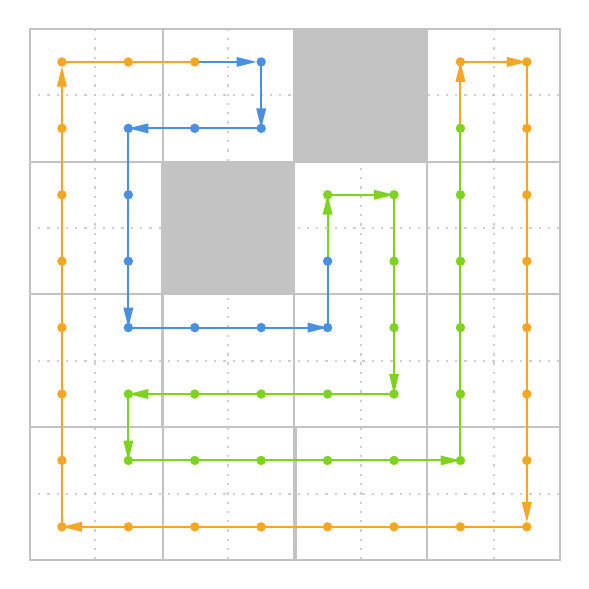
\begin{tikzpicture}[x=0.75pt,y=0.75pt,yscale=-0.8,xscale=0.8]
			%uncomment if require: \path (0,409); %set diagram left start at 0, and has height of 409
			
			%Straight Lines [id:da5351549802319371] 
			\draw [color={rgb, 255:red, 126; green, 211; blue, 33 }  ,draw opacity=1 ]   (351,195) -- (351,157) ;
			\draw [shift={(351,155)}, rotate = 450] [fill={rgb, 255:red, 126; green, 211; blue, 33 }  ,fill opacity=1 ][line width=0.08]  [draw opacity=0] (12,-3) -- (0,0) -- (12,3) -- cycle    ;
			%Straight Lines [id:da21302010090140722] 
			\draw [color={rgb, 255:red, 74; green, 144; blue, 226 }  ,draw opacity=1 ]   (271,75) -- (306.17,75) ;
			\draw [shift={(308.17,75)}, rotate = 180] [fill={rgb, 255:red, 74; green, 144; blue, 226 }  ,fill opacity=1 ][line width=0.08]  [draw opacity=0] (12,-3) -- (0,0) -- (12,3) -- cycle    ;
			%Straight Lines [id:da854517458794269] 
			\draw [color={rgb, 255:red, 195; green, 195; blue, 195 }  ,draw opacity=0.8 ] [dash pattern={on 0.84pt off 2.51pt}]  (211,55) -- (211,375) ;
			%Straight Lines [id:da5657085791005156] 
			\draw [color={rgb, 255:red, 195; green, 195; blue, 195 }  ,draw opacity=0.8 ] [dash pattern={on 0.84pt off 2.51pt}]  (291,55) -- (291,375) ;
			%Straight Lines [id:da2718901706564181] 
			\draw [color={rgb, 255:red, 195; green, 195; blue, 195 }  ,draw opacity=0.8 ] [dash pattern={on 0.84pt off 2.51pt}]  (371,55) -- (371,375) ;
			%Straight Lines [id:da02094912115129599] 
			\draw [color={rgb, 255:red, 195; green, 195; blue, 195 }  ,draw opacity=0.8 ] [dash pattern={on 0.84pt off 2.51pt}]  (451,55) -- (451,375) ;
			%Straight Lines [id:da9533932703135517] 
			\draw [color={rgb, 255:red, 195; green, 195; blue, 195 }  ,draw opacity=0.8 ] [dash pattern={on 0.84pt off 2.51pt}]  (171,95) -- (491,95) ;
			%Straight Lines [id:da9004292598975747] 
			\draw [color={rgb, 255:red, 195; green, 195; blue, 195 }  ,draw opacity=0.8 ] [dash pattern={on 0.84pt off 2.51pt}]  (171,175) -- (491,175) ;
			%Straight Lines [id:da1627688683660009] 
			\draw [color={rgb, 255:red, 195; green, 195; blue, 195 }  ,draw opacity=0.8 ] [dash pattern={on 0.84pt off 2.51pt}]  (171,255) -- (491,255) ;
			%Straight Lines [id:da4991285432755932] 
			\draw [color={rgb, 255:red, 195; green, 195; blue, 195 }  ,draw opacity=0.8 ] [dash pattern={on 0.84pt off 2.51pt}]  (171,335) -- (491,335) ;
			
			%Straight Lines [id:da7491713727663103] 
			\draw [color={rgb, 255:red, 245; green, 166; blue, 35 }  ,draw opacity=1 ]   (431,115) -- (431,77) ;
			\draw [shift={(431,75)}, rotate = 450] [fill={rgb, 255:red, 245; green, 166; blue, 35 }  ,fill opacity=1 ][line width=0.08]  [draw opacity=0] (12,-3) -- (0,0) -- (12,3) -- cycle    ;
			%Shape: Rectangle [id:dp8746081557149701] 
			\draw  [color={rgb, 255:red, 195; green, 195; blue, 195 }  ,draw opacity=1 ][line width=0.75]  (411,55) -- (491,55) -- (491,135) -- (411,135) -- cycle ;
			%Shape: Rectangle [id:dp04998372489748726] 
			\draw  [color={rgb, 255:red, 195; green, 195; blue, 195 }  ,draw opacity=1 ][line width=0.75]  (411,135) -- (491,135) -- (491,215) -- (411,215) -- cycle ;
			%Shape: Rectangle [id:dp716343211155213] 
			\draw  [color={rgb, 255:red, 195; green, 195; blue, 195 }  ,draw opacity=1 ][line width=0.75]  (411,215) -- (491,215) -- (491,295) -- (411,295) -- cycle ;
			%Shape: Rectangle [id:dp9628316526459462] 
			\draw  [color={rgb, 255:red, 195; green, 195; blue, 195 }  ,draw opacity=1 ][line width=0.75]  (411,295) -- (491,295) -- (491,375) -- (411,375) -- cycle ;
			%Shape: Rectangle [id:dp664440026053819] 
			\draw  [color={rgb, 255:red, 195; green, 195; blue, 195 }  ,draw opacity=1 ][line width=0.75]  (331,135) -- (411,135) -- (411,215) -- (331,215) -- cycle ;
			%Shape: Rectangle [id:dp08410695657353351] 
			\draw  [color={rgb, 255:red, 195; green, 195; blue, 195 }  ,draw opacity=1 ][line width=0.75]  (331,215) -- (411,215) -- (411,295) -- (331,295) -- cycle ;
			%Shape: Rectangle [id:dp07090445501331866] 
			\draw  [color={rgb, 255:red, 195; green, 195; blue, 195 }  ,draw opacity=1 ][line width=0.75]  (331,295) -- (411,295) -- (411,375) -- (331,375) -- cycle ;
			%Shape: Rectangle [id:dp8696408090436851] 
			\draw  [color={rgb, 255:red, 195; green, 195; blue, 195 }  ,draw opacity=1 ][line width=0.75]  (252,55) -- (332,55) -- (332,135) -- (252,135) -- cycle ;
			%Shape: Rectangle [id:dp4746238836207364] 
			\draw  [color={rgb, 255:red, 195; green, 195; blue, 195 }  ,draw opacity=1 ][line width=0.75]  (172,55) -- (252,55) -- (252,135) -- (172,135) -- cycle ;
			%Shape: Rectangle [id:dp8657981727821324] 
			\draw  [color={rgb, 255:red, 195; green, 195; blue, 195 }  ,draw opacity=1 ][line width=0.75]  (172,135) -- (252,135) -- (252,215) -- (172,215) -- cycle ;
			%Shape: Rectangle [id:dp20551199499502526] 
			\draw  [color={rgb, 255:red, 195; green, 195; blue, 195 }  ,draw opacity=1 ][line width=0.75]  (172,215) -- (252,215) -- (252,295) -- (172,295) -- cycle ;
			%Shape: Rectangle [id:dp5033014313679982] 
			\draw  [color={rgb, 255:red, 195; green, 195; blue, 195 }  ,draw opacity=1 ][line width=0.75]  (172,295) -- (252,295) -- (252,375) -- (172,375) -- cycle ;
			%Shape: Rectangle [id:dp0691160736423535] 
			\draw  [color={rgb, 255:red, 195; green, 195; blue, 195 }  ,draw opacity=1 ][line width=0.75]  (251,215) -- (331,215) -- (331,295) -- (251,295) -- cycle ;
			%Shape: Rectangle [id:dp9673109533181607] 
			\draw  [color={rgb, 255:red, 195; green, 195; blue, 195 }  ,draw opacity=1 ][line width=0.75]  (252,295) -- (332,295) -- (332,375) -- (252,375) -- cycle ;
			
			%Shape: Rectangle [id:dp24113727014203779] 
			\draw  [color={rgb, 255:red, 195; green, 195; blue, 195 }  ,draw opacity=1 ][fill={rgb, 255:red, 195; green, 195; blue, 195 }  ,fill opacity=1 ][line width=0.75]  (331,55) -- (411,55) -- (411,135) -- (331,135) -- cycle ;
			%Shape: Rectangle [id:dp6453850559631755] 
			\draw  [color={rgb, 255:red, 195; green, 195; blue, 195 }  ,draw opacity=1 ][fill={rgb, 255:red, 195; green, 195; blue, 195 }  ,fill opacity=1 ][line width=0.75]  (251,135) -- (331,135) -- (331,215) -- (251,215) -- cycle ;
			%Shape: Circle [id:dp6801416953242614] 
			\draw  [draw opacity=0][fill={rgb, 255:red, 245; green, 166; blue, 35 }  ,fill opacity=1 ] (468.17,75) .. controls (468.17,73.43) and (469.43,72.17) .. (471,72.17) .. controls (472.57,72.17) and (473.83,73.43) .. (473.83,75) .. controls (473.83,76.57) and (472.57,77.83) .. (471,77.83) .. controls (469.43,77.83) and (468.17,76.57) .. (468.17,75) -- cycle ;
			%Shape: Circle [id:dp4604608393759837] 
			\draw  [draw opacity=0][fill={rgb, 255:red, 245; green, 166; blue, 35 }  ,fill opacity=1 ] (428.17,75) .. controls (428.17,73.43) and (429.43,72.17) .. (431,72.17) .. controls (432.57,72.17) and (433.83,73.43) .. (433.83,75) .. controls (433.83,76.57) and (432.57,77.83) .. (431,77.83) .. controls (429.43,77.83) and (428.17,76.57) .. (428.17,75) -- cycle ;
			%Shape: Circle [id:dp13822592778240006] 
			\draw  [draw opacity=0][fill={rgb, 255:red, 245; green, 166; blue, 35 }  ,fill opacity=1 ] (468.17,115) .. controls (468.17,113.43) and (469.43,112.17) .. (471,112.17) .. controls (472.57,112.17) and (473.83,113.43) .. (473.83,115) .. controls (473.83,116.57) and (472.57,117.83) .. (471,117.83) .. controls (469.43,117.83) and (468.17,116.57) .. (468.17,115) -- cycle ;
			%Shape: Circle [id:dp544207653797784] 
			\draw  [draw opacity=0][fill={rgb, 255:red, 245; green, 166; blue, 35 }  ,fill opacity=1 ] (468.17,155) .. controls (468.17,153.43) and (469.43,152.17) .. (471,152.17) .. controls (472.57,152.17) and (473.83,153.43) .. (473.83,155) .. controls (473.83,156.57) and (472.57,157.83) .. (471,157.83) .. controls (469.43,157.83) and (468.17,156.57) .. (468.17,155) -- cycle ;
			%Shape: Circle [id:dp4171778626191891] 
			\draw  [draw opacity=0][fill={rgb, 255:red, 245; green, 166; blue, 35 }  ,fill opacity=1 ] (468.17,195) .. controls (468.17,193.43) and (469.43,192.17) .. (471,192.17) .. controls (472.57,192.17) and (473.83,193.43) .. (473.83,195) .. controls (473.83,196.57) and (472.57,197.83) .. (471,197.83) .. controls (469.43,197.83) and (468.17,196.57) .. (468.17,195) -- cycle ;
			%Shape: Circle [id:dp7895311637274933] 
			\draw  [draw opacity=0][fill={rgb, 255:red, 245; green, 166; blue, 35 }  ,fill opacity=1 ] (468.17,235) .. controls (468.17,233.43) and (469.43,232.17) .. (471,232.17) .. controls (472.57,232.17) and (473.83,233.43) .. (473.83,235) .. controls (473.83,236.57) and (472.57,237.83) .. (471,237.83) .. controls (469.43,237.83) and (468.17,236.57) .. (468.17,235) -- cycle ;
			%Shape: Circle [id:dp16643331735014688] 
			\draw  [draw opacity=0][fill={rgb, 255:red, 245; green, 166; blue, 35 }  ,fill opacity=1 ] (468.17,275) .. controls (468.17,273.43) and (469.43,272.17) .. (471,272.17) .. controls (472.57,272.17) and (473.83,273.43) .. (473.83,275) .. controls (473.83,276.57) and (472.57,277.83) .. (471,277.83) .. controls (469.43,277.83) and (468.17,276.57) .. (468.17,275) -- cycle ;
			%Shape: Circle [id:dp4612402233444193] 
			\draw  [draw opacity=0][fill={rgb, 255:red, 245; green, 166; blue, 35 }  ,fill opacity=1 ] (468.17,315) .. controls (468.17,313.43) and (469.43,312.17) .. (471,312.17) .. controls (472.57,312.17) and (473.83,313.43) .. (473.83,315) .. controls (473.83,316.57) and (472.57,317.83) .. (471,317.83) .. controls (469.43,317.83) and (468.17,316.57) .. (468.17,315) -- cycle ;
			%Shape: Circle [id:dp10168213951386096] 
			\draw  [draw opacity=0][fill={rgb, 255:red, 245; green, 166; blue, 35 }  ,fill opacity=1 ] (468.17,355) .. controls (468.17,353.43) and (469.43,352.17) .. (471,352.17) .. controls (472.57,352.17) and (473.83,353.43) .. (473.83,355) .. controls (473.83,356.57) and (472.57,357.83) .. (471,357.83) .. controls (469.43,357.83) and (468.17,356.57) .. (468.17,355) -- cycle ;
			%Shape: Circle [id:dp16583621916165892] 
			\draw  [draw opacity=0][fill={rgb, 255:red, 245; green, 166; blue, 35 }  ,fill opacity=1 ] (428.17,355) .. controls (428.17,353.43) and (429.43,352.17) .. (431,352.17) .. controls (432.57,352.17) and (433.83,353.43) .. (433.83,355) .. controls (433.83,356.57) and (432.57,357.83) .. (431,357.83) .. controls (429.43,357.83) and (428.17,356.57) .. (428.17,355) -- cycle ;
			%Shape: Circle [id:dp23056644975317875] 
			\draw  [draw opacity=0][fill={rgb, 255:red, 245; green, 166; blue, 35 }  ,fill opacity=1 ] (388.17,355) .. controls (388.17,353.43) and (389.43,352.17) .. (391,352.17) .. controls (392.57,352.17) and (393.83,353.43) .. (393.83,355) .. controls (393.83,356.57) and (392.57,357.83) .. (391,357.83) .. controls (389.43,357.83) and (388.17,356.57) .. (388.17,355) -- cycle ;
			%Shape: Circle [id:dp8401836553855346] 
			\draw  [draw opacity=0][fill={rgb, 255:red, 245; green, 166; blue, 35 }  ,fill opacity=1 ] (348.17,355) .. controls (348.17,353.43) and (349.43,352.17) .. (351,352.17) .. controls (352.57,352.17) and (353.83,353.43) .. (353.83,355) .. controls (353.83,356.57) and (352.57,357.83) .. (351,357.83) .. controls (349.43,357.83) and (348.17,356.57) .. (348.17,355) -- cycle ;
			%Shape: Circle [id:dp48282190307261685] 
			\draw  [draw opacity=0][fill={rgb, 255:red, 245; green, 166; blue, 35 }  ,fill opacity=1 ] (308.17,355) .. controls (308.17,353.43) and (309.43,352.17) .. (311,352.17) .. controls (312.57,352.17) and (313.83,353.43) .. (313.83,355) .. controls (313.83,356.57) and (312.57,357.83) .. (311,357.83) .. controls (309.43,357.83) and (308.17,356.57) .. (308.17,355) -- cycle ;
			%Shape: Circle [id:dp5761975450405177] 
			\draw  [draw opacity=0][fill={rgb, 255:red, 245; green, 166; blue, 35 }  ,fill opacity=1 ] (268.17,355) .. controls (268.17,353.43) and (269.43,352.17) .. (271,352.17) .. controls (272.57,352.17) and (273.83,353.43) .. (273.83,355) .. controls (273.83,356.57) and (272.57,357.83) .. (271,357.83) .. controls (269.43,357.83) and (268.17,356.57) .. (268.17,355) -- cycle ;
			%Shape: Circle [id:dp06870423995803909] 
			\draw  [draw opacity=0][fill={rgb, 255:red, 245; green, 166; blue, 35 }  ,fill opacity=1 ] (228.17,355) .. controls (228.17,353.43) and (229.43,352.17) .. (231,352.17) .. controls (232.57,352.17) and (233.83,353.43) .. (233.83,355) .. controls (233.83,356.57) and (232.57,357.83) .. (231,357.83) .. controls (229.43,357.83) and (228.17,356.57) .. (228.17,355) -- cycle ;
			%Shape: Circle [id:dp5381906142714585] 
			\draw  [draw opacity=0][fill={rgb, 255:red, 245; green, 166; blue, 35 }  ,fill opacity=1 ] (188.17,355) .. controls (188.17,353.43) and (189.43,352.17) .. (191,352.17) .. controls (192.57,352.17) and (193.83,353.43) .. (193.83,355) .. controls (193.83,356.57) and (192.57,357.83) .. (191,357.83) .. controls (189.43,357.83) and (188.17,356.57) .. (188.17,355) -- cycle ;
			%Shape: Circle [id:dp03637900283495887] 
			\draw  [draw opacity=0][fill={rgb, 255:red, 245; green, 166; blue, 35 }  ,fill opacity=1 ] (188.17,315) .. controls (188.17,313.43) and (189.43,312.17) .. (191,312.17) .. controls (192.57,312.17) and (193.83,313.43) .. (193.83,315) .. controls (193.83,316.57) and (192.57,317.83) .. (191,317.83) .. controls (189.43,317.83) and (188.17,316.57) .. (188.17,315) -- cycle ;
			%Shape: Circle [id:dp5512808090993917] 
			\draw  [draw opacity=0][fill={rgb, 255:red, 245; green, 166; blue, 35 }  ,fill opacity=1 ] (188.17,275) .. controls (188.17,273.43) and (189.43,272.17) .. (191,272.17) .. controls (192.57,272.17) and (193.83,273.43) .. (193.83,275) .. controls (193.83,276.57) and (192.57,277.83) .. (191,277.83) .. controls (189.43,277.83) and (188.17,276.57) .. (188.17,275) -- cycle ;
			%Shape: Circle [id:dp7146308141223112] 
			\draw  [draw opacity=0][fill={rgb, 255:red, 245; green, 166; blue, 35 }  ,fill opacity=1 ] (188.17,235) .. controls (188.17,233.43) and (189.43,232.17) .. (191,232.17) .. controls (192.57,232.17) and (193.83,233.43) .. (193.83,235) .. controls (193.83,236.57) and (192.57,237.83) .. (191,237.83) .. controls (189.43,237.83) and (188.17,236.57) .. (188.17,235) -- cycle ;
			%Shape: Circle [id:dp5335478422961473] 
			\draw  [draw opacity=0][fill={rgb, 255:red, 245; green, 166; blue, 35 }  ,fill opacity=1 ] (188.17,195) .. controls (188.17,193.43) and (189.43,192.17) .. (191,192.17) .. controls (192.57,192.17) and (193.83,193.43) .. (193.83,195) .. controls (193.83,196.57) and (192.57,197.83) .. (191,197.83) .. controls (189.43,197.83) and (188.17,196.57) .. (188.17,195) -- cycle ;
			%Shape: Circle [id:dp8716915789137862] 
			\draw  [draw opacity=0][fill={rgb, 255:red, 245; green, 166; blue, 35 }  ,fill opacity=1 ] (188.17,155) .. controls (188.17,153.43) and (189.43,152.17) .. (191,152.17) .. controls (192.57,152.17) and (193.83,153.43) .. (193.83,155) .. controls (193.83,156.57) and (192.57,157.83) .. (191,157.83) .. controls (189.43,157.83) and (188.17,156.57) .. (188.17,155) -- cycle ;
			%Shape: Circle [id:dp3349585094431857] 
			\draw  [draw opacity=0][fill={rgb, 255:red, 245; green, 166; blue, 35 }  ,fill opacity=1 ] (188.17,115) .. controls (188.17,113.43) and (189.43,112.17) .. (191,112.17) .. controls (192.57,112.17) and (193.83,113.43) .. (193.83,115) .. controls (193.83,116.57) and (192.57,117.83) .. (191,117.83) .. controls (189.43,117.83) and (188.17,116.57) .. (188.17,115) -- cycle ;
			%Shape: Circle [id:dp44273518739120976] 
			\draw  [draw opacity=0][fill={rgb, 255:red, 245; green, 166; blue, 35 }  ,fill opacity=1 ] (188.17,75) .. controls (188.17,73.43) and (189.43,72.17) .. (191,72.17) .. controls (192.57,72.17) and (193.83,73.43) .. (193.83,75) .. controls (193.83,76.57) and (192.57,77.83) .. (191,77.83) .. controls (189.43,77.83) and (188.17,76.57) .. (188.17,75) -- cycle ;
			%Shape: Circle [id:dp8508549485124735] 
			\draw  [draw opacity=0][fill={rgb, 255:red, 245; green, 166; blue, 35 }  ,fill opacity=1 ] (228.17,75) .. controls (228.17,73.43) and (229.43,72.17) .. (231,72.17) .. controls (232.57,72.17) and (233.83,73.43) .. (233.83,75) .. controls (233.83,76.57) and (232.57,77.83) .. (231,77.83) .. controls (229.43,77.83) and (228.17,76.57) .. (228.17,75) -- cycle ;
			%Shape: Circle [id:dp6783308931260619] 
			\draw  [draw opacity=0][fill={rgb, 255:red, 245; green, 166; blue, 35 }  ,fill opacity=1 ] (268.17,75) .. controls (268.17,73.43) and (269.43,72.17) .. (271,72.17) .. controls (272.57,72.17) and (273.83,73.43) .. (273.83,75) .. controls (273.83,76.57) and (272.57,77.83) .. (271,77.83) .. controls (269.43,77.83) and (268.17,76.57) .. (268.17,75) -- cycle ;
			%Straight Lines [id:da5456587577326129] 
			\draw [color={rgb, 255:red, 245; green, 166; blue, 35 }  ,draw opacity=1 ]   (431,75) -- (469,75) ;
			\draw [shift={(471,75)}, rotate = 180] [fill={rgb, 255:red, 245; green, 166; blue, 35 }  ,fill opacity=1 ][line width=0.08]  [draw opacity=0] (12,-3) -- (0,0) -- (12,3) -- cycle    ;
			%Shape: Circle [id:dp4443238058444041] 
			\draw  [draw opacity=0][fill={rgb, 255:red, 74; green, 144; blue, 226 }  ,fill opacity=1 ] (308.17,75) .. controls (308.17,73.43) and (309.43,72.17) .. (311,72.17) .. controls (312.57,72.17) and (313.83,73.43) .. (313.83,75) .. controls (313.83,76.57) and (312.57,77.83) .. (311,77.83) .. controls (309.43,77.83) and (308.17,76.57) .. (308.17,75) -- cycle ;
			%Shape: Circle [id:dp29010302295723345] 
			\draw  [draw opacity=0][fill={rgb, 255:red, 74; green, 144; blue, 226 }  ,fill opacity=1 ] (308.17,115) .. controls (308.17,113.43) and (309.43,112.17) .. (311,112.17) .. controls (312.57,112.17) and (313.83,113.43) .. (313.83,115) .. controls (313.83,116.57) and (312.57,117.83) .. (311,117.83) .. controls (309.43,117.83) and (308.17,116.57) .. (308.17,115) -- cycle ;
			%Shape: Circle [id:dp6216098523896874] 
			\draw  [draw opacity=0][fill={rgb, 255:red, 74; green, 144; blue, 226 }  ,fill opacity=1 ] (268.17,115) .. controls (268.17,113.43) and (269.43,112.17) .. (271,112.17) .. controls (272.57,112.17) and (273.83,113.43) .. (273.83,115) .. controls (273.83,116.57) and (272.57,117.83) .. (271,117.83) .. controls (269.43,117.83) and (268.17,116.57) .. (268.17,115) -- cycle ;
			%Shape: Circle [id:dp06234830362754895] 
			\draw  [draw opacity=0][fill={rgb, 255:red, 74; green, 144; blue, 226 }  ,fill opacity=1 ] (228.17,115) .. controls (228.17,113.43) and (229.43,112.17) .. (231,112.17) .. controls (232.57,112.17) and (233.83,113.43) .. (233.83,115) .. controls (233.83,116.57) and (232.57,117.83) .. (231,117.83) .. controls (229.43,117.83) and (228.17,116.57) .. (228.17,115) -- cycle ;
			%Shape: Circle [id:dp9885173496004662] 
			\draw  [draw opacity=0][fill={rgb, 255:red, 74; green, 144; blue, 226 }  ,fill opacity=1 ] (228.17,155) .. controls (228.17,153.43) and (229.43,152.17) .. (231,152.17) .. controls (232.57,152.17) and (233.83,153.43) .. (233.83,155) .. controls (233.83,156.57) and (232.57,157.83) .. (231,157.83) .. controls (229.43,157.83) and (228.17,156.57) .. (228.17,155) -- cycle ;
			%Shape: Circle [id:dp9444674235776642] 
			\draw  [draw opacity=0][fill={rgb, 255:red, 74; green, 144; blue, 226 }  ,fill opacity=1 ] (228.17,195) .. controls (228.17,193.43) and (229.43,192.17) .. (231,192.17) .. controls (232.57,192.17) and (233.83,193.43) .. (233.83,195) .. controls (233.83,196.57) and (232.57,197.83) .. (231,197.83) .. controls (229.43,197.83) and (228.17,196.57) .. (228.17,195) -- cycle ;
			%Shape: Circle [id:dp7868027408873275] 
			\draw  [draw opacity=0][fill={rgb, 255:red, 74; green, 144; blue, 226 }  ,fill opacity=1 ] (228.17,235) .. controls (228.17,233.43) and (229.43,232.17) .. (231,232.17) .. controls (232.57,232.17) and (233.83,233.43) .. (233.83,235) .. controls (233.83,236.57) and (232.57,237.83) .. (231,237.83) .. controls (229.43,237.83) and (228.17,236.57) .. (228.17,235) -- cycle ;
			%Shape: Circle [id:dp35955963628126275] 
			\draw  [draw opacity=0][fill={rgb, 255:red, 74; green, 144; blue, 226 }  ,fill opacity=1 ] (268.17,235) .. controls (268.17,233.43) and (269.43,232.17) .. (271,232.17) .. controls (272.57,232.17) and (273.83,233.43) .. (273.83,235) .. controls (273.83,236.57) and (272.57,237.83) .. (271,237.83) .. controls (269.43,237.83) and (268.17,236.57) .. (268.17,235) -- cycle ;
			%Shape: Circle [id:dp5516376120857398] 
			\draw  [draw opacity=0][fill={rgb, 255:red, 74; green, 144; blue, 226 }  ,fill opacity=1 ] (308.17,235) .. controls (308.17,233.43) and (309.43,232.17) .. (311,232.17) .. controls (312.57,232.17) and (313.83,233.43) .. (313.83,235) .. controls (313.83,236.57) and (312.57,237.83) .. (311,237.83) .. controls (309.43,237.83) and (308.17,236.57) .. (308.17,235) -- cycle ;
			%Shape: Circle [id:dp5893700740487555] 
			\draw  [draw opacity=0][fill={rgb, 255:red, 74; green, 144; blue, 226 }  ,fill opacity=1 ] (348.17,235) .. controls (348.17,233.43) and (349.43,232.17) .. (351,232.17) .. controls (352.57,232.17) and (353.83,233.43) .. (353.83,235) .. controls (353.83,236.57) and (352.57,237.83) .. (351,237.83) .. controls (349.43,237.83) and (348.17,236.57) .. (348.17,235) -- cycle ;
			%Shape: Circle [id:dp1286587461477784] 
			\draw  [draw opacity=0][fill={rgb, 255:red, 74; green, 144; blue, 226 }  ,fill opacity=1 ] (348.17,195) .. controls (348.17,193.43) and (349.43,192.17) .. (351,192.17) .. controls (352.57,192.17) and (353.83,193.43) .. (353.83,195) .. controls (353.83,196.57) and (352.57,197.83) .. (351,197.83) .. controls (349.43,197.83) and (348.17,196.57) .. (348.17,195) -- cycle ;
			%Shape: Circle [id:dp26088941378322006] 
			\draw  [draw opacity=0][fill={rgb, 255:red, 126; green, 211; blue, 33 }  ,fill opacity=1 ] (348.17,155) .. controls (348.17,153.43) and (349.43,152.17) .. (351,152.17) .. controls (352.57,152.17) and (353.83,153.43) .. (353.83,155) .. controls (353.83,156.57) and (352.57,157.83) .. (351,157.83) .. controls (349.43,157.83) and (348.17,156.57) .. (348.17,155) -- cycle ;
			%Shape: Circle [id:dp9676514649936712] 
			\draw  [draw opacity=0][fill={rgb, 255:red, 126; green, 211; blue, 33 }  ,fill opacity=1 ] (388.17,155) .. controls (388.17,153.43) and (389.43,152.17) .. (391,152.17) .. controls (392.57,152.17) and (393.83,153.43) .. (393.83,155) .. controls (393.83,156.57) and (392.57,157.83) .. (391,157.83) .. controls (389.43,157.83) and (388.17,156.57) .. (388.17,155) -- cycle ;
			%Shape: Circle [id:dp19213789582339302] 
			\draw  [draw opacity=0][fill={rgb, 255:red, 126; green, 211; blue, 33 }  ,fill opacity=1 ] (388.17,195) .. controls (388.17,193.43) and (389.43,192.17) .. (391,192.17) .. controls (392.57,192.17) and (393.83,193.43) .. (393.83,195) .. controls (393.83,196.57) and (392.57,197.83) .. (391,197.83) .. controls (389.43,197.83) and (388.17,196.57) .. (388.17,195) -- cycle ;
			%Shape: Circle [id:dp31757377829209155] 
			\draw  [draw opacity=0][fill={rgb, 255:red, 126; green, 211; blue, 33 }  ,fill opacity=1 ] (388.17,235) .. controls (388.17,233.43) and (389.43,232.17) .. (391,232.17) .. controls (392.57,232.17) and (393.83,233.43) .. (393.83,235) .. controls (393.83,236.57) and (392.57,237.83) .. (391,237.83) .. controls (389.43,237.83) and (388.17,236.57) .. (388.17,235) -- cycle ;
			%Shape: Circle [id:dp11411146161431085] 
			\draw  [draw opacity=0][fill={rgb, 255:red, 126; green, 211; blue, 33 }  ,fill opacity=1 ] (388.17,275) .. controls (388.17,273.43) and (389.43,272.17) .. (391,272.17) .. controls (392.57,272.17) and (393.83,273.43) .. (393.83,275) .. controls (393.83,276.57) and (392.57,277.83) .. (391,277.83) .. controls (389.43,277.83) and (388.17,276.57) .. (388.17,275) -- cycle ;
			%Shape: Circle [id:dp6075376860133745] 
			\draw  [draw opacity=0][fill={rgb, 255:red, 126; green, 211; blue, 33 }  ,fill opacity=1 ] (348.17,275) .. controls (348.17,273.43) and (349.43,272.17) .. (351,272.17) .. controls (352.57,272.17) and (353.83,273.43) .. (353.83,275) .. controls (353.83,276.57) and (352.57,277.83) .. (351,277.83) .. controls (349.43,277.83) and (348.17,276.57) .. (348.17,275) -- cycle ;
			%Shape: Circle [id:dp33787943985666535] 
			\draw  [draw opacity=0][fill={rgb, 255:red, 126; green, 211; blue, 33 }  ,fill opacity=1 ] (308.17,275) .. controls (308.17,273.43) and (309.43,272.17) .. (311,272.17) .. controls (312.57,272.17) and (313.83,273.43) .. (313.83,275) .. controls (313.83,276.57) and (312.57,277.83) .. (311,277.83) .. controls (309.43,277.83) and (308.17,276.57) .. (308.17,275) -- cycle ;
			%Shape: Circle [id:dp6967659869352532] 
			\draw  [draw opacity=0][fill={rgb, 255:red, 126; green, 211; blue, 33 }  ,fill opacity=1 ] (268.17,275) .. controls (268.17,273.43) and (269.43,272.17) .. (271,272.17) .. controls (272.57,272.17) and (273.83,273.43) .. (273.83,275) .. controls (273.83,276.57) and (272.57,277.83) .. (271,277.83) .. controls (269.43,277.83) and (268.17,276.57) .. (268.17,275) -- cycle ;
			%Shape: Circle [id:dp7916368779271419] 
			\draw  [draw opacity=0][fill={rgb, 255:red, 126; green, 211; blue, 33 }  ,fill opacity=1 ] (228.17,275) .. controls (228.17,273.43) and (229.43,272.17) .. (231,272.17) .. controls (232.57,272.17) and (233.83,273.43) .. (233.83,275) .. controls (233.83,276.57) and (232.57,277.83) .. (231,277.83) .. controls (229.43,277.83) and (228.17,276.57) .. (228.17,275) -- cycle ;
			%Shape: Circle [id:dp9131057577477717] 
			\draw  [draw opacity=0][fill={rgb, 255:red, 126; green, 211; blue, 33 }  ,fill opacity=1 ] (228.17,315) .. controls (228.17,313.43) and (229.43,312.17) .. (231,312.17) .. controls (232.57,312.17) and (233.83,313.43) .. (233.83,315) .. controls (233.83,316.57) and (232.57,317.83) .. (231,317.83) .. controls (229.43,317.83) and (228.17,316.57) .. (228.17,315) -- cycle ;
			%Shape: Circle [id:dp060540910098607625] 
			\draw  [draw opacity=0][fill={rgb, 255:red, 126; green, 211; blue, 33 }  ,fill opacity=1 ] (268.17,315) .. controls (268.17,313.43) and (269.43,312.17) .. (271,312.17) .. controls (272.57,312.17) and (273.83,313.43) .. (273.83,315) .. controls (273.83,316.57) and (272.57,317.83) .. (271,317.83) .. controls (269.43,317.83) and (268.17,316.57) .. (268.17,315) -- cycle ;
			%Shape: Circle [id:dp4358067111786901] 
			\draw  [draw opacity=0][fill={rgb, 255:red, 126; green, 211; blue, 33 }  ,fill opacity=1 ] (308.17,315) .. controls (308.17,313.43) and (309.43,312.17) .. (311,312.17) .. controls (312.57,312.17) and (313.83,313.43) .. (313.83,315) .. controls (313.83,316.57) and (312.57,317.83) .. (311,317.83) .. controls (309.43,317.83) and (308.17,316.57) .. (308.17,315) -- cycle ;
			%Shape: Circle [id:dp6562545880538291] 
			\draw  [draw opacity=0][fill={rgb, 255:red, 126; green, 211; blue, 33 }  ,fill opacity=1 ] (348.17,315) .. controls (348.17,313.43) and (349.43,312.17) .. (351,312.17) .. controls (352.57,312.17) and (353.83,313.43) .. (353.83,315) .. controls (353.83,316.57) and (352.57,317.83) .. (351,317.83) .. controls (349.43,317.83) and (348.17,316.57) .. (348.17,315) -- cycle ;
			%Shape: Circle [id:dp18058415370378111] 
			\draw  [draw opacity=0][fill={rgb, 255:red, 126; green, 211; blue, 33 }  ,fill opacity=1 ] (388.17,315) .. controls (388.17,313.43) and (389.43,312.17) .. (391,312.17) .. controls (392.57,312.17) and (393.83,313.43) .. (393.83,315) .. controls (393.83,316.57) and (392.57,317.83) .. (391,317.83) .. controls (389.43,317.83) and (388.17,316.57) .. (388.17,315) -- cycle ;
			%Shape: Circle [id:dp10115316904907612] 
			\draw  [draw opacity=0][fill={rgb, 255:red, 126; green, 211; blue, 33 }  ,fill opacity=1 ] (428.17,315) .. controls (428.17,313.43) and (429.43,312.17) .. (431,312.17) .. controls (432.57,312.17) and (433.83,313.43) .. (433.83,315) .. controls (433.83,316.57) and (432.57,317.83) .. (431,317.83) .. controls (429.43,317.83) and (428.17,316.57) .. (428.17,315) -- cycle ;
			%Shape: Circle [id:dp835742083306757] 
			\draw  [draw opacity=0][fill={rgb, 255:red, 126; green, 211; blue, 33 }  ,fill opacity=1 ] (428.17,275) .. controls (428.17,273.43) and (429.43,272.17) .. (431,272.17) .. controls (432.57,272.17) and (433.83,273.43) .. (433.83,275) .. controls (433.83,276.57) and (432.57,277.83) .. (431,277.83) .. controls (429.43,277.83) and (428.17,276.57) .. (428.17,275) -- cycle ;
			%Shape: Circle [id:dp780791295796917] 
			\draw  [draw opacity=0][fill={rgb, 255:red, 126; green, 211; blue, 33 }  ,fill opacity=1 ] (428.17,235) .. controls (428.17,233.43) and (429.43,232.17) .. (431,232.17) .. controls (432.57,232.17) and (433.83,233.43) .. (433.83,235) .. controls (433.83,236.57) and (432.57,237.83) .. (431,237.83) .. controls (429.43,237.83) and (428.17,236.57) .. (428.17,235) -- cycle ;
			%Shape: Circle [id:dp742197015069753] 
			\draw  [draw opacity=0][fill={rgb, 255:red, 126; green, 211; blue, 33 }  ,fill opacity=1 ] (428.17,195) .. controls (428.17,193.43) and (429.43,192.17) .. (431,192.17) .. controls (432.57,192.17) and (433.83,193.43) .. (433.83,195) .. controls (433.83,196.57) and (432.57,197.83) .. (431,197.83) .. controls (429.43,197.83) and (428.17,196.57) .. (428.17,195) -- cycle ;
			%Shape: Circle [id:dp058172723888363365] 
			\draw  [draw opacity=0][fill={rgb, 255:red, 126; green, 211; blue, 33 }  ,fill opacity=1 ] (428.17,155) .. controls (428.17,153.43) and (429.43,152.17) .. (431,152.17) .. controls (432.57,152.17) and (433.83,153.43) .. (433.83,155) .. controls (433.83,156.57) and (432.57,157.83) .. (431,157.83) .. controls (429.43,157.83) and (428.17,156.57) .. (428.17,155) -- cycle ;
			%Shape: Circle [id:dp40603445670354055] 
			\draw  [draw opacity=0][fill={rgb, 255:red, 126; green, 211; blue, 33 }  ,fill opacity=1 ] (428.17,115) .. controls (428.17,113.43) and (429.43,112.17) .. (431,112.17) .. controls (432.57,112.17) and (433.83,113.43) .. (433.83,115) .. controls (433.83,116.57) and (432.57,117.83) .. (431,117.83) .. controls (429.43,117.83) and (428.17,116.57) .. (428.17,115) -- cycle ;
			%Straight Lines [id:da16789636771970073] 
			\draw [color={rgb, 255:red, 245; green, 166; blue, 35 }  ,draw opacity=1 ]   (471,75) -- (471,350.17) ;
			\draw [shift={(471,352.17)}, rotate = 270] [fill={rgb, 255:red, 245; green, 166; blue, 35 }  ,fill opacity=1 ][line width=0.08]  [draw opacity=0] (12,-3) -- (0,0) -- (12,3) -- cycle    ;
			%Straight Lines [id:da3449631876846895] 
			\draw [color={rgb, 255:red, 245; green, 166; blue, 35 }  ,draw opacity=1 ]   (471,355) -- (193,355) ;
			\draw [shift={(191,355)}, rotate = 360] [fill={rgb, 255:red, 245; green, 166; blue, 35 }  ,fill opacity=1 ][line width=0.08]  [draw opacity=0] (12,-3) -- (0,0) -- (12,3) -- cycle    ;
			%Straight Lines [id:da10161365475922346] 
			\draw [color={rgb, 255:red, 245; green, 166; blue, 35 }  ,draw opacity=1 ]   (191,355) -- (191,79.83) ;
			\draw [shift={(191,77.83)}, rotate = 450] [fill={rgb, 255:red, 245; green, 166; blue, 35 }  ,fill opacity=1 ][line width=0.08]  [draw opacity=0] (12,-3) -- (0,0) -- (12,3) -- cycle    ;
			%Straight Lines [id:da8632021686141709] 
			\draw [color={rgb, 255:red, 245; green, 166; blue, 35 }  ,draw opacity=1 ]   (191,75) -- (271,75) ;
			%Straight Lines [id:da7671632448461922] 
			\draw [color={rgb, 255:red, 74; green, 144; blue, 226 }  ,draw opacity=1 ]   (311,75) -- (311,113) ;
			\draw [shift={(311,115)}, rotate = 270] [fill={rgb, 255:red, 74; green, 144; blue, 226 }  ,fill opacity=1 ][line width=0.08]  [draw opacity=0] (12,-3) -- (0,0) -- (12,3) -- cycle    ;
			%Straight Lines [id:da672307594730295] 
			\draw [color={rgb, 255:red, 74; green, 144; blue, 226 }  ,draw opacity=1 ]   (311,115) -- (233,115) ;
			\draw [shift={(231,115)}, rotate = 360] [fill={rgb, 255:red, 74; green, 144; blue, 226 }  ,fill opacity=1 ][line width=0.08]  [draw opacity=0] (12,-3) -- (0,0) -- (12,3) -- cycle    ;
			%Straight Lines [id:da4077834871044419] 
			\draw [color={rgb, 255:red, 74; green, 144; blue, 226 }  ,draw opacity=1 ]   (231,115) -- (231,233) ;
			\draw [shift={(231,235)}, rotate = 270] [fill={rgb, 255:red, 74; green, 144; blue, 226 }  ,fill opacity=1 ][line width=0.08]  [draw opacity=0] (12,-3) -- (0,0) -- (12,3) -- cycle    ;
			%Straight Lines [id:da9346944539277193] 
			\draw [color={rgb, 255:red, 74; green, 144; blue, 226 }  ,draw opacity=1 ]   (231,235) -- (349,235) ;
			\draw [shift={(351,235)}, rotate = 180] [fill={rgb, 255:red, 74; green, 144; blue, 226 }  ,fill opacity=1 ][line width=0.08]  [draw opacity=0] (12,-3) -- (0,0) -- (12,3) -- cycle    ;
			%Straight Lines [id:da6701207435426635] 
			\draw [color={rgb, 255:red, 74; green, 144; blue, 226 }  ,draw opacity=1 ]   (351,235) -- (351,195) ;
			%Straight Lines [id:da5501151214452311] 
			\draw [color={rgb, 255:red, 126; green, 211; blue, 33 }  ,draw opacity=1 ]   (351,155) -- (389,155) ;
			\draw [shift={(391,155)}, rotate = 180] [fill={rgb, 255:red, 126; green, 211; blue, 33 }  ,fill opacity=1 ][line width=0.08]  [draw opacity=0] (12,-3) -- (0,0) -- (12,3) -- cycle    ;
			%Straight Lines [id:da4311911132527191] 
			\draw [color={rgb, 255:red, 126; green, 211; blue, 33 }  ,draw opacity=1 ]   (391,155) -- (391,194) -- (391,273) ;
			\draw [shift={(391,275)}, rotate = 270] [fill={rgb, 255:red, 126; green, 211; blue, 33 }  ,fill opacity=1 ][line width=0.08]  [draw opacity=0] (12,-3) -- (0,0) -- (12,3) -- cycle    ;
			%Straight Lines [id:da5705388383279479] 
			\draw [color={rgb, 255:red, 126; green, 211; blue, 33 }  ,draw opacity=1 ]   (391,275) -- (233,275) ;
			\draw [shift={(231,275)}, rotate = 360] [fill={rgb, 255:red, 126; green, 211; blue, 33 }  ,fill opacity=1 ][line width=0.08]  [draw opacity=0] (12,-3) -- (0,0) -- (12,3) -- cycle    ;
			%Straight Lines [id:da21297417889995085] 
			\draw [color={rgb, 255:red, 126; green, 211; blue, 33 }  ,draw opacity=1 ]   (231,275) -- (231,313) ;
			\draw [shift={(231,315)}, rotate = 270] [fill={rgb, 255:red, 126; green, 211; blue, 33 }  ,fill opacity=1 ][line width=0.08]  [draw opacity=0] (12,-3) -- (0,0) -- (12,3) -- cycle    ;
			%Straight Lines [id:da22819451965736026] 
			\draw [color={rgb, 255:red, 126; green, 211; blue, 33 }  ,draw opacity=1 ]   (231,315) -- (429,315) ;
			\draw [shift={(431,315)}, rotate = 180] [fill={rgb, 255:red, 126; green, 211; blue, 33 }  ,fill opacity=1 ][line width=0.08]  [draw opacity=0] (12,-3) -- (0,0) -- (12,3) -- cycle    ;
			%Straight Lines [id:da7504973565926707] 
			\draw [color={rgb, 255:red, 126; green, 211; blue, 33 }  ,draw opacity=1 ]   (431,315) -- (431,115) ;
			
			
			
			
		\end{tikzpicture}
		\caption{Path generated by generating way-points from arrows}
		\label{fig:wpnts01}
	\end{subfigure}
	\hfill
	\begin{subfigure}{0.45\textwidth}
		\centering
		\tikzset{every picture/.style={line width=0.75pt}} %set default line width to 0.75pt        
		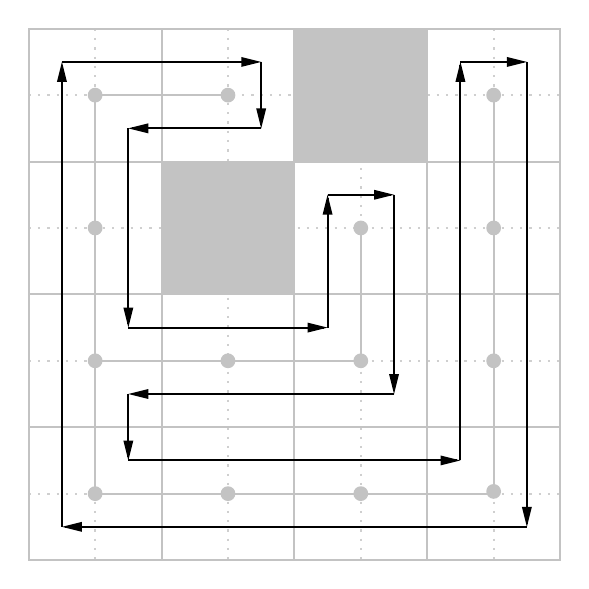
\begin{tikzpicture}[x=0.75pt,y=0.75pt,yscale=-0.8,xscale=0.8]
			%uncomment if require: \path (0,401); %set diagram left start at 0, and has height of 401
			
			%Straight Lines [id:da6525656097654802] 
			\draw [color={rgb, 255:red, 195; green, 195; blue, 195 }  ,draw opacity=0.8 ] [dash pattern={on 0.84pt off 2.51pt}]  (209,36) -- (209,356) ;
			%Straight Lines [id:da9449615822379405] 
			\draw [color={rgb, 255:red, 195; green, 195; blue, 195 }  ,draw opacity=0.8 ] [dash pattern={on 0.84pt off 2.51pt}]  (289,36) -- (289,356) ;
			%Straight Lines [id:da49922694692753367] 
			\draw [color={rgb, 255:red, 195; green, 195; blue, 195 }  ,draw opacity=0.8 ] [dash pattern={on 0.84pt off 2.51pt}]  (369,36) -- (369,356) ;
			%Straight Lines [id:da42403625075839124] 
			\draw [color={rgb, 255:red, 195; green, 195; blue, 195 }  ,draw opacity=0.8 ] [dash pattern={on 0.84pt off 2.51pt}]  (449,36) -- (449,356) ;
			%Straight Lines [id:da41382258883228107] 
			\draw [color={rgb, 255:red, 195; green, 195; blue, 195 }  ,draw opacity=0.8 ] [dash pattern={on 0.84pt off 2.51pt}]  (169,76) -- (489,76) ;
			%Straight Lines [id:da37487046166351323] 
			\draw [color={rgb, 255:red, 195; green, 195; blue, 195 }  ,draw opacity=0.8 ] [dash pattern={on 0.84pt off 2.51pt}]  (169,156) -- (489,156) ;
			%Straight Lines [id:da7805503540839331] 
			\draw [color={rgb, 255:red, 195; green, 195; blue, 195 }  ,draw opacity=0.8 ] [dash pattern={on 0.84pt off 2.51pt}]  (169,236) -- (489,236) ;
			%Straight Lines [id:da0007847063653105835] 
			\draw [color={rgb, 255:red, 195; green, 195; blue, 195 }  ,draw opacity=0.8 ] [dash pattern={on 0.84pt off 2.51pt}]  (169,316) -- (489,316) ;
			
			%Shape: Rectangle [id:dp9282250935920651] 
			\draw  [color={rgb, 255:red, 195; green, 195; blue, 195 }  ,draw opacity=1 ][line width=0.75]  (409,36) -- (489,36) -- (489,116) -- (409,116) -- cycle ;
			%Shape: Rectangle [id:dp40889920048446493] 
			\draw  [color={rgb, 255:red, 195; green, 195; blue, 195 }  ,draw opacity=1 ][line width=0.75]  (409,116) -- (489,116) -- (489,196) -- (409,196) -- cycle ;
			%Shape: Rectangle [id:dp08210856469103622] 
			\draw  [color={rgb, 255:red, 195; green, 195; blue, 195 }  ,draw opacity=1 ][line width=0.75]  (409,196) -- (489,196) -- (489,276) -- (409,276) -- cycle ;
			%Shape: Rectangle [id:dp11132018353927009] 
			\draw  [color={rgb, 255:red, 195; green, 195; blue, 195 }  ,draw opacity=1 ][line width=0.75]  (409,276) -- (489,276) -- (489,356) -- (409,356) -- cycle ;
			%Shape: Rectangle [id:dp056079390985070976] 
			\draw  [color={rgb, 255:red, 195; green, 195; blue, 195 }  ,draw opacity=1 ][line width=0.75]  (329,116) -- (409,116) -- (409,196) -- (329,196) -- cycle ;
			%Shape: Rectangle [id:dp8717884780085985] 
			\draw  [color={rgb, 255:red, 195; green, 195; blue, 195 }  ,draw opacity=1 ][line width=0.75]  (329,196) -- (409,196) -- (409,276) -- (329,276) -- cycle ;
			%Shape: Rectangle [id:dp6966702207831605] 
			\draw  [color={rgb, 255:red, 195; green, 195; blue, 195 }  ,draw opacity=1 ][line width=0.75]  (329,276) -- (409,276) -- (409,356) -- (329,356) -- cycle ;
			%Shape: Rectangle [id:dp6557240237758346] 
			\draw  [color={rgb, 255:red, 195; green, 195; blue, 195 }  ,draw opacity=1 ][line width=0.75]  (249,36) -- (329,36) -- (329,116) -- (249,116) -- cycle ;
			%Shape: Rectangle [id:dp46922355033620544] 
			\draw  [color={rgb, 255:red, 195; green, 195; blue, 195 }  ,draw opacity=1 ][line width=0.75]  (169,36) -- (249,36) -- (249,116) -- (169,116) -- cycle ;
			%Shape: Rectangle [id:dp7130641235448705] 
			\draw  [color={rgb, 255:red, 195; green, 195; blue, 195 }  ,draw opacity=1 ][line width=0.75]  (169,116) -- (249,116) -- (249,196) -- (169,196) -- cycle ;
			%Shape: Rectangle [id:dp8416366697669087] 
			\draw  [color={rgb, 255:red, 195; green, 195; blue, 195 }  ,draw opacity=1 ][line width=0.75]  (169,196) -- (249,196) -- (249,276) -- (169,276) -- cycle ;
			%Shape: Rectangle [id:dp5912644819544948] 
			\draw  [color={rgb, 255:red, 195; green, 195; blue, 195 }  ,draw opacity=1 ][line width=0.75]  (169,276) -- (249,276) -- (249,356) -- (169,356) -- cycle ;
			%Shape: Rectangle [id:dp6447358006368811] 
			\draw  [color={rgb, 255:red, 195; green, 195; blue, 195 }  ,draw opacity=1 ][line width=0.75]  (249,196) -- (329,196) -- (329,276) -- (249,276) -- cycle ;
			%Shape: Rectangle [id:dp8887506508423009] 
			\draw  [color={rgb, 255:red, 195; green, 195; blue, 195 }  ,draw opacity=1 ][line width=0.75]  (249,276) -- (329,276) -- (329,356) -- (249,356) -- cycle ;
			
			%Straight Lines [id:da1738948188181435] 
			\draw [color={rgb, 255:red, 195; green, 195; blue, 195 }  ,draw opacity=1 ]   (209,76) -- (265,76) -- (289,76) ;
			%Straight Lines [id:da7049505215325911] 
			\draw [color={rgb, 255:red, 195; green, 195; blue, 195 }  ,draw opacity=1 ]   (209,76) -- (209,316) ;
			%Straight Lines [id:da9869392385512394] 
			\draw [color={rgb, 255:red, 195; green, 195; blue, 195 }  ,draw opacity=1 ]   (209,316) -- (449,316) ;
			%Straight Lines [id:da1614981151805881] 
			\draw [color={rgb, 255:red, 195; green, 195; blue, 195 }  ,draw opacity=1 ]   (449,77) -- (449,317) ;
			%Straight Lines [id:da45917613825264225] 
			\draw [color={rgb, 255:red, 195; green, 195; blue, 195 }  ,draw opacity=1 ]   (369,237) -- (369,157) ;
			%Straight Lines [id:da6889780670091039] 
			\draw [color={rgb, 255:red, 195; green, 195; blue, 195 }  ,draw opacity=1 ]   (209,236) -- (369,236) ;
			%Straight Lines [id:da12273195124066882] 
			\draw [color={rgb, 255:red, 0; green, 0; blue, 0 }  ,draw opacity=1 ][fill={rgb, 255:red, 0; green, 0; blue, 0 }  ,fill opacity=1 ]   (349,216) -- (349,138) ;
			\draw [shift={(349,136)}, rotate = 450] [fill={rgb, 255:red, 0; green, 0; blue, 0 }  ,fill opacity=1 ][line width=0.08]  [draw opacity=0] (12,-3) -- (0,0) -- (12,3) -- cycle    ;
			%Straight Lines [id:da3917937162075191] 
			\draw [color={rgb, 255:red, 0; green, 0; blue, 0 }  ,draw opacity=1 ][fill={rgb, 255:red, 0; green, 0; blue, 0 }  ,fill opacity=1 ]   (229,216) -- (347,216) ;
			\draw [shift={(349,216)}, rotate = 180] [fill={rgb, 255:red, 0; green, 0; blue, 0 }  ,fill opacity=1 ][line width=0.08]  [draw opacity=0] (12,-3) -- (0,0) -- (12,3) -- cycle    ;
			%Straight Lines [id:da4803441771366592] 
			\draw [color={rgb, 255:red, 0; green, 0; blue, 0 }  ,draw opacity=1 ][fill={rgb, 255:red, 0; green, 0; blue, 0 }  ,fill opacity=1 ]   (229,96) -- (229,214) ;
			\draw [shift={(229,216)}, rotate = 270] [fill={rgb, 255:red, 0; green, 0; blue, 0 }  ,fill opacity=1 ][line width=0.08]  [draw opacity=0] (12,-3) -- (0,0) -- (12,3) -- cycle    ;
			%Straight Lines [id:da7402482792888903] 
			\draw [color={rgb, 255:red, 0; green, 0; blue, 0 }  ,draw opacity=1 ][fill={rgb, 255:red, 0; green, 0; blue, 0 }  ,fill opacity=1 ]   (309,96) -- (231,96) ;
			\draw [shift={(229,96)}, rotate = 360] [fill={rgb, 255:red, 0; green, 0; blue, 0 }  ,fill opacity=1 ][line width=0.08]  [draw opacity=0] (12,-3) -- (0,0) -- (12,3) -- cycle    ;
			%Straight Lines [id:da8948623102095223] 
			\draw [color={rgb, 255:red, 0; green, 0; blue, 0 }  ,draw opacity=1 ][fill={rgb, 255:red, 0; green, 0; blue, 0 }  ,fill opacity=1 ]   (309,56) -- (309,94) ;
			\draw [shift={(309,96)}, rotate = 270] [fill={rgb, 255:red, 0; green, 0; blue, 0 }  ,fill opacity=1 ][line width=0.08]  [draw opacity=0] (12,-3) -- (0,0) -- (12,3) -- cycle    ;
			%Straight Lines [id:da25998808169222265] 
			\draw [color={rgb, 255:red, 0; green, 0; blue, 0 }  ,draw opacity=1 ][fill={rgb, 255:red, 0; green, 0; blue, 0 }  ,fill opacity=1 ]   (189,56) -- (307,56) ;
			\draw [shift={(309,56)}, rotate = 180] [fill={rgb, 255:red, 0; green, 0; blue, 0 }  ,fill opacity=1 ][line width=0.08]  [draw opacity=0] (12,-3) -- (0,0) -- (12,3) -- cycle    ;
			%Straight Lines [id:da40263375664736256] 
			\draw [color={rgb, 255:red, 0; green, 0; blue, 0 }  ,draw opacity=1 ][fill={rgb, 255:red, 0; green, 0; blue, 0 }  ,fill opacity=1 ]   (189,336) -- (189,58) ;
			\draw [shift={(189,56)}, rotate = 450] [fill={rgb, 255:red, 0; green, 0; blue, 0 }  ,fill opacity=1 ][line width=0.08]  [draw opacity=0] (12,-3) -- (0,0) -- (12,3) -- cycle    ;
			%Straight Lines [id:da48570875534448854] 
			\draw [color={rgb, 255:red, 0; green, 0; blue, 0 }  ,draw opacity=1 ][fill={rgb, 255:red, 0; green, 0; blue, 0 }  ,fill opacity=1 ]   (469,336) -- (191,336) ;
			\draw [shift={(189,336)}, rotate = 360] [fill={rgb, 255:red, 0; green, 0; blue, 0 }  ,fill opacity=1 ][line width=0.08]  [draw opacity=0] (12,-3) -- (0,0) -- (12,3) -- cycle    ;
			%Straight Lines [id:da8647185294436568] 
			\draw [color={rgb, 255:red, 0; green, 0; blue, 0 }  ,draw opacity=1 ][fill={rgb, 255:red, 0; green, 0; blue, 0 }  ,fill opacity=1 ]   (469,56) -- (469,334) ;
			\draw [shift={(469,336)}, rotate = 270] [fill={rgb, 255:red, 0; green, 0; blue, 0 }  ,fill opacity=1 ][line width=0.08]  [draw opacity=0] (12,-3) -- (0,0) -- (12,3) -- cycle    ;
			%Straight Lines [id:da5962728530510046] 
			\draw [color={rgb, 255:red, 0; green, 0; blue, 0 }  ,draw opacity=1 ][fill={rgb, 255:red, 0; green, 0; blue, 0 }  ,fill opacity=1 ]   (429,296) -- (429,58) ;
			\draw [shift={(429,56)}, rotate = 450] [fill={rgb, 255:red, 0; green, 0; blue, 0 }  ,fill opacity=1 ][line width=0.08]  [draw opacity=0] (12,-3) -- (0,0) -- (12,3) -- cycle    ;
			%Straight Lines [id:da3206966034529801] 
			\draw [color={rgb, 255:red, 0; green, 0; blue, 0 }  ,draw opacity=1 ][fill={rgb, 255:red, 0; green, 0; blue, 0 }  ,fill opacity=1 ]   (229,296) -- (427,296) ;
			\draw [shift={(429,296)}, rotate = 180] [fill={rgb, 255:red, 0; green, 0; blue, 0 }  ,fill opacity=1 ][line width=0.08]  [draw opacity=0] (12,-3) -- (0,0) -- (12,3) -- cycle    ;
			%Shape: Rectangle [id:dp2343107393386883] 
			\draw  [color={rgb, 255:red, 195; green, 195; blue, 195 }  ,draw opacity=1 ][fill={rgb, 255:red, 195; green, 195; blue, 195 }  ,fill opacity=1 ][line width=0.75]  (329,36) -- (409,36) -- (409,116) -- (329,116) -- cycle ;
			%Shape: Rectangle [id:dp7923981711361026] 
			\draw  [color={rgb, 255:red, 195; green, 195; blue, 195 }  ,draw opacity=1 ][fill={rgb, 255:red, 195; green, 195; blue, 195 }  ,fill opacity=1 ][line width=0.75]  (249,116) -- (329,116) -- (329,196) -- (249,196) -- cycle ;
			%Straight Lines [id:da8657248227410601] 
			\draw [color={rgb, 255:red, 0; green, 0; blue, 0 }  ,draw opacity=1 ][fill={rgb, 255:red, 0; green, 0; blue, 0 }  ,fill opacity=1 ]   (429,56) -- (467,56) ;
			\draw [shift={(469,56)}, rotate = 180] [fill={rgb, 255:red, 0; green, 0; blue, 0 }  ,fill opacity=1 ][line width=0.08]  [draw opacity=0] (12,-3) -- (0,0) -- (12,3) -- cycle    ;
			%Straight Lines [id:da6481028434657641] 
			\draw [color={rgb, 255:red, 0; green, 0; blue, 0 }  ,draw opacity=1 ][fill={rgb, 255:red, 0; green, 0; blue, 0 }  ,fill opacity=1 ]   (349,136) -- (387,136) ;
			\draw [shift={(389,136)}, rotate = 180] [fill={rgb, 255:red, 0; green, 0; blue, 0 }  ,fill opacity=1 ][line width=0.08]  [draw opacity=0] (12,-3) -- (0,0) -- (12,3) -- cycle    ;
			%Straight Lines [id:da16504553800477284] 
			\draw [color={rgb, 255:red, 0; green, 0; blue, 0 }  ,draw opacity=1 ][fill={rgb, 255:red, 0; green, 0; blue, 0 }  ,fill opacity=1 ]   (389,136) -- (389,176) -- (389,254) ;
			\draw [shift={(389,256)}, rotate = 270] [fill={rgb, 255:red, 0; green, 0; blue, 0 }  ,fill opacity=1 ][line width=0.08]  [draw opacity=0] (12,-3) -- (0,0) -- (12,3) -- cycle    ;
			%Straight Lines [id:da6863050610327999] 
			\draw [color={rgb, 255:red, 0; green, 0; blue, 0 }  ,draw opacity=1 ][fill={rgb, 255:red, 0; green, 0; blue, 0 }  ,fill opacity=1 ]   (389,256) -- (231,256) ;
			\draw [shift={(229,256)}, rotate = 360] [fill={rgb, 255:red, 0; green, 0; blue, 0 }  ,fill opacity=1 ][line width=0.08]  [draw opacity=0] (12,-3) -- (0,0) -- (12,3) -- cycle    ;
			%Straight Lines [id:da621163023150217] 
			\draw [color={rgb, 255:red, 0; green, 0; blue, 0 }  ,draw opacity=1 ][fill={rgb, 255:red, 0; green, 0; blue, 0 }  ,fill opacity=1 ]   (229,256) -- (229,294) ;
			\draw [shift={(229,296)}, rotate = 270] [fill={rgb, 255:red, 0; green, 0; blue, 0 }  ,fill opacity=1 ][line width=0.08]  [draw opacity=0] (12,-3) -- (0,0) -- (12,3) -- cycle    ;
			%Shape: Circle [id:dp35079329412457416] 
			\draw  [color={rgb, 255:red, 195; green, 195; blue, 195 }  ,draw opacity=1 ][fill={rgb, 255:red, 195; green, 195; blue, 195 }  ,fill opacity=1 ] (285.19,76) .. controls (285.19,73.89) and (286.89,72.19) .. (289,72.19) .. controls (291.11,72.19) and (292.81,73.89) .. (292.81,76) .. controls (292.81,78.11) and (291.11,79.81) .. (289,79.81) .. controls (286.89,79.81) and (285.19,78.11) .. (285.19,76) -- cycle ;
			%Shape: Circle [id:dp9648717674150975] 
			\draw  [color={rgb, 255:red, 195; green, 195; blue, 195 }  ,draw opacity=1 ][fill={rgb, 255:red, 195; green, 195; blue, 195 }  ,fill opacity=1 ] (205.19,76) .. controls (205.19,73.89) and (206.89,72.19) .. (209,72.19) .. controls (211.11,72.19) and (212.81,73.89) .. (212.81,76) .. controls (212.81,78.11) and (211.11,79.81) .. (209,79.81) .. controls (206.89,79.81) and (205.19,78.11) .. (205.19,76) -- cycle ;
			%Shape: Circle [id:dp7643919500463263] 
			\draw  [color={rgb, 255:red, 195; green, 195; blue, 195 }  ,draw opacity=1 ][fill={rgb, 255:red, 195; green, 195; blue, 195 }  ,fill opacity=1 ] (205.19,156) .. controls (205.19,153.89) and (206.89,152.19) .. (209,152.19) .. controls (211.11,152.19) and (212.81,153.89) .. (212.81,156) .. controls (212.81,158.11) and (211.11,159.81) .. (209,159.81) .. controls (206.89,159.81) and (205.19,158.11) .. (205.19,156) -- cycle ;
			%Shape: Circle [id:dp3452724725015799] 
			\draw  [color={rgb, 255:red, 195; green, 195; blue, 195 }  ,draw opacity=1 ][fill={rgb, 255:red, 195; green, 195; blue, 195 }  ,fill opacity=1 ] (205.19,236) .. controls (205.19,233.89) and (206.89,232.19) .. (209,232.19) .. controls (211.11,232.19) and (212.81,233.89) .. (212.81,236) .. controls (212.81,238.11) and (211.11,239.81) .. (209,239.81) .. controls (206.89,239.81) and (205.19,238.11) .. (205.19,236) -- cycle ;
			%Shape: Circle [id:dp9410421155127517] 
			\draw  [color={rgb, 255:red, 195; green, 195; blue, 195 }  ,draw opacity=1 ][fill={rgb, 255:red, 195; green, 195; blue, 195 }  ,fill opacity=1 ] (285.19,236) .. controls (285.19,233.89) and (286.89,232.19) .. (289,232.19) .. controls (291.11,232.19) and (292.81,233.89) .. (292.81,236) .. controls (292.81,238.11) and (291.11,239.81) .. (289,239.81) .. controls (286.89,239.81) and (285.19,238.11) .. (285.19,236) -- cycle ;
			%Shape: Circle [id:dp8706824138912068] 
			\draw  [color={rgb, 255:red, 195; green, 195; blue, 195 }  ,draw opacity=1 ][fill={rgb, 255:red, 195; green, 195; blue, 195 }  ,fill opacity=1 ] (365.19,236) .. controls (365.19,233.89) and (366.89,232.19) .. (369,232.19) .. controls (371.11,232.19) and (372.81,233.89) .. (372.81,236) .. controls (372.81,238.11) and (371.11,239.81) .. (369,239.81) .. controls (366.89,239.81) and (365.19,238.11) .. (365.19,236) -- cycle ;
			%Shape: Circle [id:dp6741904628479463] 
			\draw  [color={rgb, 255:red, 195; green, 195; blue, 195 }  ,draw opacity=1 ][fill={rgb, 255:red, 195; green, 195; blue, 195 }  ,fill opacity=1 ] (365.19,156) .. controls (365.19,153.89) and (366.89,152.19) .. (369,152.19) .. controls (371.11,152.19) and (372.81,153.89) .. (372.81,156) .. controls (372.81,158.11) and (371.11,159.81) .. (369,159.81) .. controls (366.89,159.81) and (365.19,158.11) .. (365.19,156) -- cycle ;
			%Shape: Circle [id:dp7682685511530534] 
			\draw  [color={rgb, 255:red, 195; green, 195; blue, 195 }  ,draw opacity=1 ][fill={rgb, 255:red, 195; green, 195; blue, 195 }  ,fill opacity=1 ] (205.19,316) .. controls (205.19,313.89) and (206.89,312.19) .. (209,312.19) .. controls (211.11,312.19) and (212.81,313.89) .. (212.81,316) .. controls (212.81,318.11) and (211.11,319.81) .. (209,319.81) .. controls (206.89,319.81) and (205.19,318.11) .. (205.19,316) -- cycle ;
			%Shape: Circle [id:dp9360991155818204] 
			\draw  [color={rgb, 255:red, 195; green, 195; blue, 195 }  ,draw opacity=1 ][fill={rgb, 255:red, 195; green, 195; blue, 195 }  ,fill opacity=1 ] (285.19,316) .. controls (285.19,313.89) and (286.89,312.19) .. (289,312.19) .. controls (291.11,312.19) and (292.81,313.89) .. (292.81,316) .. controls (292.81,318.11) and (291.11,319.81) .. (289,319.81) .. controls (286.89,319.81) and (285.19,318.11) .. (285.19,316) -- cycle ;
			%Shape: Circle [id:dp02784897953102572] 
			\draw  [color={rgb, 255:red, 195; green, 195; blue, 195 }  ,draw opacity=1 ][fill={rgb, 255:red, 195; green, 195; blue, 195 }  ,fill opacity=1 ] (365.19,316) .. controls (365.19,313.89) and (366.89,312.19) .. (369,312.19) .. controls (371.11,312.19) and (372.81,313.89) .. (372.81,316) .. controls (372.81,318.11) and (371.11,319.81) .. (369,319.81) .. controls (366.89,319.81) and (365.19,318.11) .. (365.19,316) -- cycle ;
			%Shape: Circle [id:dp25399764324655116] 
			\draw  [color={rgb, 255:red, 195; green, 195; blue, 195 }  ,draw opacity=1 ][fill={rgb, 255:red, 195; green, 195; blue, 195 }  ,fill opacity=1 ] (445.19,314.67) .. controls (445.19,312.56) and (446.89,310.85) .. (449,310.85) .. controls (451.11,310.85) and (452.81,312.56) .. (452.81,314.67) .. controls (452.81,316.77) and (451.11,318.48) .. (449,318.48) .. controls (446.89,318.48) and (445.19,316.77) .. (445.19,314.67) -- cycle ;
			%Shape: Circle [id:dp34699799070971116] 
			\draw  [color={rgb, 255:red, 195; green, 195; blue, 195 }  ,draw opacity=1 ][fill={rgb, 255:red, 195; green, 195; blue, 195 }  ,fill opacity=1 ] (445.19,236) .. controls (445.19,233.89) and (446.89,232.19) .. (449,232.19) .. controls (451.11,232.19) and (452.81,233.89) .. (452.81,236) .. controls (452.81,238.11) and (451.11,239.81) .. (449,239.81) .. controls (446.89,239.81) and (445.19,238.11) .. (445.19,236) -- cycle ;
			%Shape: Circle [id:dp139463928707797] 
			\draw  [color={rgb, 255:red, 195; green, 195; blue, 195 }  ,draw opacity=1 ][fill={rgb, 255:red, 195; green, 195; blue, 195 }  ,fill opacity=1 ] (445.19,156) .. controls (445.19,153.89) and (446.89,152.19) .. (449,152.19) .. controls (451.11,152.19) and (452.81,153.89) .. (452.81,156) .. controls (452.81,158.11) and (451.11,159.81) .. (449,159.81) .. controls (446.89,159.81) and (445.19,158.11) .. (445.19,156) -- cycle ;
			%Shape: Circle [id:dp6433117239923425] 
			\draw  [color={rgb, 255:red, 195; green, 195; blue, 195 }  ,draw opacity=1 ][fill={rgb, 255:red, 195; green, 195; blue, 195 }  ,fill opacity=1 ] (445.19,76) .. controls (445.19,73.89) and (446.89,72.19) .. (449,72.19) .. controls (451.11,72.19) and (452.81,73.89) .. (452.81,76) .. controls (452.81,78.11) and (451.11,79.81) .. (449,79.81) .. controls (446.89,79.81) and (445.19,78.11) .. (445.19,76) -- cycle ;
		\end{tikzpicture}
		\caption{Resulting circumnavigation path around spanning tree}
		\label{fig:wpnts02}
	\end{subfigure}
	\caption{Figures showing way-points generated from arrows along with the resulting circumnavigation path around the spanning tree.}
\end{figure}

The resulting path achieves full coverage of the environment, provided the \ac{uav} follows it exactly. The assumption here is that the camera footprint will cover the cell when the \ac{uav} enters that cell. 
% Refer back to conceptualisation and modelling here. What error is allowed on the path.
% Is this achievable by normal UAVs (NO) -> Dynamic constraints

\section{Spanning Tree Weights}
\section{Spanning Tree Coverage with DARP}
% Illustrative Results